%________________________________________________________________________________________________

\chapter{Introduction}

\section{Motivation}

\subsection{Why concurrency and time matter}

In the world we live in, concurrency is ubiquitous. Imagine that we are walking inside a forest. Different birds, animals and insects are talking around us. Suddenly we see a beautiful bird peeping from a branch of a sunlit mossy tree. Our brain here is processing multiple sensory information, motor control, and cognition concurrently. Images, sounds, movement, forming memories, making a decision whether to capture this moment in our camera or not--- all are processed concurrently by different parts of our brain. At the same time, our heart rate, breathing, and reflexes are being controlled by other parts. These processes evolve largely independently, yet remain sufficiently coordinated to produce coherent behaviour. Such parallel activity illustrates a fundamental property of natural systems: concurrency. 

Natural systems rarely operate sequentially. Cellular processes, ecosystem dynamics, and social interactions all exhibit intrinsic concurrency. In contrast, engineered systems were historically designed from a sequential viewpoint. Modern applications, however—such as autonomous vehicles, medical devices, communication protocols, and industrial automation—are inherently concurrent and distributed. These informal examples motivate the need for mathematical models that capture independent yet coordinated evolution of system components.

Many such systems are also time-critical. For instance, in automotive systems, a collision avoidance controller may process camera data every \(33\) ms and radar data every \(50\) ms, while requiring sensor fusion within a tight deadline to trigger braking. Pacemakers coordinate several concurrent processes that monitor heart rhythm, detect arrhythmias, and deliver electrical impulses with microsecond precision. In telecommunication networks, multiple radio channels operate concurrently while maintaining stringent timing synchronization, and in industrial assembly lines multiple robotic arms must synchronize their movements to avoid collisions. In such settings, timing is not merely an auxiliary attribute, but a determining factor for correctness.

These examples illustrate systems where both \emph{concurrency} and \emph{quantitative timing} are essential for correctness. Moreover, the interactions between components are often \emph{multiparty}: three or more processes must synchronize simultaneously. Classical models of concurrency tend to reduce multiparty interactions to sequences of binary communications, obscuring the true structure of the system. This thesis explores a model that takes multiparty synchronization as primitive: \emph{local-timed negotiations}.

\subsection{Verification and the Reachability Problem}

In time-critical concurrent systems, even small malfunctions can have catastrophic consequences, leading to loss of life, environmental damage, or severe financial losses. This highlights the practical imperative behind the formal study of concurrent systems. The theoretical motivation lies in developing mathematical theories for new areas of interest. 

\emph{Formal verification} aims to establish algorithmically whether a system satisfies a specification. The central question is: given a system model $S$ and a specification $\mathit{spec}$ (such as a safety property), does the behavior of $S$ satisfy $\mathit{spec}$, written $S \models \mathit{spec}$?

One of the most fundamental verification problems is \emph{reachability}: can the system transition from an initial configuration to a particular target configuration? Reachability captures many important properties:
\begin{itemize}
\item \textbf{Safety}: Can the system reach an error state?
\item \textbf{Deadlock-freedom}: Can the system reach a state where no progress is possible?
\item \textbf{Goal reachability}: Can the system reach a desired goal state?
\end{itemize}

\textit{Reachability analysis}, a core building block of many verification tasks, is determining whether a system can transition from an initial configuration to a specific target configuration (state, location, or marking). For example, when verifying safety properties, one often asks whether any ``bad'' state is reachable from the initial state. If not, the safety property is satisfied.

For untimed concurrent systems, reachability is often decidable but computationally expensive. The main obstacle is \emph{state-space explosion}: even small systems can have enormous numbers of reachable states due to the many possible interleavings of concurrent actions. \emph{Partial-order reduction} (POR) techniques address this by exploiting independence: if two actions affect disjoint parts of the system state, we need not explore all their interleavings. However, extending POR to timed models is challenging. In networks of timed automata, for example, clocks induce implicit synchronization between actions that would otherwise be independent, complicating independence checks. This implicit synchronization is a major obstacle to applying partial-order reduction techniques in timed-concurrent systems. One of the motivations behind negotiation-based models is precisely to expose independence and true concurrency more explicitly, which suggests new opportunities for partial-order reasoning even in the presence of time.

\subsection{Historical background and local-timed negotiations}

Although concurrent systems abound, no single unifying mathematical model for concurrency has emerged that plays a role fully analogous to that of Turing machines or the $\lambda$-calculus for sequential computation. Several models of concurrency have been proposed, including Petri nets, process algebras, asynchronous automata, and Mazurkiewicz traces, each emphasizing different aspects such as causality, communication, or synchronization.

Negotiations~\cite{EsparzaDeselNegotiations} are among the more recent models that take concurrency as a primitive notion. Unlike Petri nets, negotiations take atomic multiparty synchronization as a primitive, rather than encoding it indirectly via places and transitions. On the other hand, \textit{timed automata}~\cite{AlurDillTA} provide a widely used formalism for modelling real-time systems with clock constraints, and are the foundation of several verification tools. It is therefore natural to study \textit{timed versions of negotiations}, combining the rich concurrency structure of negotiations with quantitative timing constraints.

%In this thesis, we study a real-time extension of negotiations known as \textit{local-timed negotiations} (LTNs), where each agent maintains its own local time, and some interactions may synchronize these local clocks. The key distinguishing feature is that time is inherently local to agents, rather than global, and synchronization is an explicit modelling choice rather than an implicit consequence of shared clocks. This setting allows us to explore the interaction between concurrency, partial synchrony, and quantitative timing constraints, and to understand their impact on reachability and verification.

\paragraph{Thesis overview and contributions.}
This thesis studies the \emph{reachability problem} for \emph{local-timed negotiations} (LTNs), a model of concurrent systems that combines atomic multiparty synchronization with quantitative timing constraints and local clocks. In contrast to classical timed automata, time in LTNs is inherently local to agents, and synchronization of time is an explicit modelling choice rather than an implicit consequence of shared clocks. This explicit separation between local time evolution and synchronization exposes true concurrency and independence in timed systems.

We show that allowing arbitrary mixtures of time-synchronizing and non-synchronizing interactions leads to undecidability of reachability, by encoding unbounded computation using local clocks and selective synchronization. To recover decidability, we identify several structural and semantic restrictions under which reachability becomes decidable and PSPACE-complete. These include synchronization-free LTNs, fully-synchronizing LTNs, drift-bounded LTNs—where the difference between local times of agents remains bounded—and connectedly-communicating LTNs, where repeated synchronization enforces bounded drift along cycles. Together, these results provide a systematic landscape of decidability and complexity for reachability in local-timed negotiations, clarifying the precise role played by synchronization and local time in concurrent real-time systems.

%__________________________________________________________________________________

\section{Timed automata, reachability, and negotiations}
\label{sec:intro-models}

The central problem addressed in this thesis is the \emph{reachability problem for local-timed negotiations}: given an initial configuration and a target location (or marking, depending on the variant), does there exist an execution that reaches the target while respecting local timing constraints? Understanding the decidability and complexity of this problem is essential for assessing the suitability of local-timed negotiations as a verification model. Before introducing local-timed negotiations, we review reachability for timed automata and then recall the underlying (untimed) negotiation model with an illustrative example.

We will formalize local-timed negotiations in Chapter~\ref{chap:ltn}. In this section, we first revisit the reachability problem for timed automata, and then describe negotiations and their reachability problem.

\subsection{Timed automata}
\label{subsec:ta-reachability}

A \emph{timed automaton}~\cite{AlurDillTA} is a finite-state automaton equipped with a finite set of non-negative real-valued variables called \emph{clocks}. Clocks evolve continuously and synchronously with global time, and can be compared to integer constants in transition guards and reset to \(0\) when transitions are taken. Formally, a transition is labelled with:
\begin{itemize}
  \item an input symbol,
  \item a \emph{guard}, which is a conjunction of atomic constraints of the form \(x \bowtie c\) where \(x\) is a clock, \(c \in \mathbb{N}\), and \(\bowtie \in \{\le,<,\ge,>\}\),
  \item and a set of clocks to be reset.
\end{itemize}
A transition is enabled when the current clock valuation satisfies its guard. The automaton has a designated initial state and a set of accepting (or target) states. We restrict attention to the standard Alur–Dill model with integer constants and without diagonal constraints, which suffices for our purposes.

Figure~\ref{fig:ab} shows an example timed automaton \(\mathcal{A}_1\) with two clocks \(x\) and \(y\), initial state \(q_0\), accepting state \(q_2\), and alphabet \(\{a,b\}\).

\begin{figure}[t]
\centering
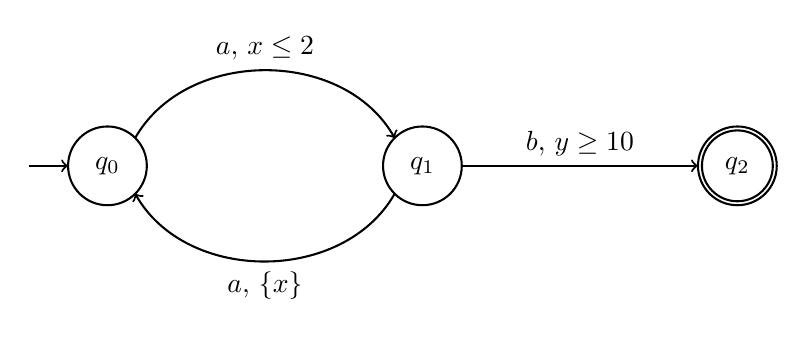
\begin{tikzpicture}[scale=1, every node/.style={transform shape}]

\filldraw [fill=white]  (0,0)  circle (5mm) node (q0) {$q_0$};
\filldraw [fill=white]  (4,0)  circle (5mm) node (q1) {$q_1$};
\filldraw [fill=white]  (8,0)  circle (5mm) node (q2) {$q_2$};
\draw (8,0)  circle (4.5mm);

\begin{scope}[->]
\draw (0.35,0.35) .. controls (1,1.5) and (3,1.5) .. (3.65,0.35) node [midway, above] {$a,\, x \leq 2$};
\draw (3.65,-0.35) .. controls (3,-1.5) and (1,-1.5) .. (0.35,-0.35) node [midway, below] {$a,\, \{x\}$};
\draw (4.5,0) -- (7.5,0) node [midway, above] {$b,\, y \geq 10$};
\draw (-1,0) -- (-0.5,0);
\end{scope}

\end{tikzpicture}
\caption{A timed automaton \(\mathcal{A}_1\). Both clocks \(x\) and \(y\) start at \(0\) in state \(q_0\). The transition on \(a\) from \(q_0\) to \(q_1\) has the guard \(x \leq 2\), forcing the system to spend at most \(2\) time units before taking it. The transition on \(a\) from \(q_1\) to \(q_0\) has no guard and resets \(x\). The guard on \(b\) from \(q_1\) to \(q_2\) requires that at least \(10\) time units have elapsed since the start, via the constraint \(y \geq 10\).}
\label{fig:ab}
\end{figure}

\paragraph{Semantics and State Space.}
A configuration of a timed automaton is a pair \((q,v)\) where \(q\) is a location and \(v\) is a valuation assigning to each clock a non-negative real number. Timed automata have two kinds of transitions:
\begin{itemize}
  \item \emph{Delay transitions}, where time elapses and all clocks increase uniformly.
  \item \emph{Action transitions}, where a guarded transition is fired and some clocks are reset.
\end{itemize}

\begin{figure}[t]
\centering
\begin{tikzpicture}

\node at (0,0) {$(q_0, \langle 0, 0 \rangle)$};
\node at (-4,-2) {$(q_1, \langle 0, 0 \rangle)$};
\node at (0,-2) {$(q_1, \langle 0.8, 0.8 \rangle)$};
\node at (4,-2) {$(q_1, \langle 1.5, 1.5 \rangle)$};
\node at (-4,-4) {$(q_0, \langle 0, 0.8 \rangle)$};
\node at (0,-4) {$(q_0, \langle 0, 5.8 \rangle)$};
\node at (4,-4) {$(q_0, \langle 0, 9.8 \rangle)$};
\node at (0,-6) {$(q_1, \langle 0.5, 10.3 \rangle)$};
\node at (4,-6) {$(q_1, \langle 1.2, 11 \rangle)$};
\node at (8,-6) {$(q_1, \langle 1.8, 11.6  \rangle)$};
\node at (4,-8) {$(q_2, \langle 2.2, 12 \rangle)$};

\node at (-2,-2) {$\cdots$};
\node at (2,-2) {$\cdots$};
\node at (6,-2) {$\cdots$};
\node at (-2,-4) {$\cdots$};
\node at (2,-4) {$\cdots$};
\node at (6,-4) {$\cdots$};
\node at (-2,-6) {$\cdots$};
\node at (2,-6) {$\cdots$};
\node at (6,-6) {$\cdots$};
\node at (10,-6) {$\cdots$};
\node at (2,-8) {$\cdots$};
\node at (6,-8) {$\cdots$};
\node at (-4,-2.5) {$\vdots$};
\node at (4,-2.5) {$\vdots$};
\node at (-4,-4.5) {$\vdots$};
\node at (0,-4.5) {$\vdots$};
\node at (0,-6.5) {$\vdots$};
\node at (8,-6.5) {$\vdots$};

\begin{scope}[-Stealth]
\draw (0,-0.3) -- (-4,-1.7) node [midway, left, above] {\footnotesize $0$};
\draw (0,-0.3) -- (0,-1.7) node [midway, left] {\footnotesize $0.8$};
\draw (0,-0.3) -- (4,-1.7) node [midway, right, above] {\footnotesize $1.5$};
\draw (0,-2.3) -- (-4,-3.7) node [midway, left, above] {\footnotesize $0$};
\draw (0,-2.3) -- (0,-3.7) node [midway, left] {\footnotesize $5$};
\draw (0,-2.3) -- (4,-3.7) node [midway, right, above] {\footnotesize $9$};
\draw (4,-4.3) -- (0,-5.7) node [midway, left, above] {\footnotesize $0.5$};
\draw (4,-4.3) -- (4,-5.7) node [midway, left] {\footnotesize $1.2$};
\draw (4,-4.3) -- (8,-5.7) node [midway, right, above] {\footnotesize $1.8$};
\draw (4,-6.3) -- (4,-7.7) node [midway, left] {\footnotesize $1$};
\end{scope}

\end{tikzpicture}
\caption{Part of the transition system of the timed automaton \(\mathcal{A}_1\), showing several possible runs.}
\label{fig:ab-behavior}
\end{figure}

Figure~\ref{fig:ab-behavior} depicts part of the (infinite) transition system of \(\mathcal{A}_1\), showing some possible configurations and transitions. Starting from the initial configuration \((q_0, \langle 0,0 \rangle)\), the system may let time elapse in \(q_0\) for any duration between \(0\) and \(2\) units before taking the transition on \(a\) to \(q_1\). For instance, after \(0.8\) time units, the clock valuation becomes \(\langle 0.8, 0.8 \rangle\). Once in \(q_1\), the automaton can again delay, and may take the loop on \(a\) (resetting \(x\)) or eventually take the transition on \(b\) when \(y \ge 10\). Different choices of delay durations lead to uncountably many distinct runs.

\paragraph{The Reachability Problem and Its Solutions.}
The \emph{reachability problem} for a timed automaton asks whether there exists a run from the initial state to an accepting state. Reachability has been extensively studied and forms the basis of verification tools such as \textsc{UPPAAL}, \textsc{Kronos}, \textsc{TChecker}, and \textsc{Theta}.

A key difficulty is that the space of clock valuations is uncountable. For any fixed sequence of action transitions, there are uncountably many ways to interleave delays, leading to uncountably many runs. To solve the reachability problem effectively, one must reason symbolically about sets of valuations.

The classical solution relies on a finite partition of the valuation space into equivalence classes called \emph{regions}~\cite{AlurDillTA}. Given a bound function \(M\) that associates to each clock \(x\) the largest constant appearing in any guard involving \(x\), one defines a finite partition where clock valuations in the same region are indistinguishable with respect to reachability. For the automaton \(\mathcal{A}_1\), the maximal bound function \(M_1\) satisfies \(M_1(x) = 2\) and \(M_1(y) = 10\). The \emph{region graph} is then obtained by taking the product of locations with regions. It has been shown that the region graph is sound and complete for reachability~\cite{AlurDillTA}. However, region graphs are often too large to be practical for verification.

In practice, reachability analysis for timed automata is typically based on \emph{zones}~\cite{DillPhD} rather than regions. Zones are convex sets of clock valuations defined by difference constraints of the form \(x - y \bowtie c\). They can be efficiently represented and manipulated using difference bound matrices (DBMs), yielding scalable algorithms. In this thesis, we will rely on regions as a conceptual tool to reason about finiteness and complexity, but our main focus will be on modelling and complexity rather than implementing zone-based algorithms.

\paragraph{Networks of Timed Automata.} Real systems often consist of multiple concurrent components, modeled as networks of timed automata that synchronize on shared actions. In the standard semantics, all automata share a global time, and their clocks advance synchronously. This global-time assumption simplifies some aspects of verification but obscures potential independence between components.

\subsection{Negotiations}
\label{subsubsec:negotiations}

Where timed automata focus on individual agents with timing constraints, \emph{negotiations}~\cite{EsparzaDeselNegotiations} provide a model of concurrency centered on multiparty synchronization. A negotiation structures workflow as atomic multiparty interactions. We give an informal description here; the precise definition is recalled in Chapter \ref{chap:preliminaries}. A multiparty \emph{atomic negotiation} involves a set of \emph{processes} (or \emph{agents}) jointly choosing an outcome from a finite set. Esparza and Desel introduced \emph{distributed negotiations} (or simply \emph{negotiations})~\cite{EsparzaDeselNegotiations} as a model of concurrency where such atomic negotiations are the basic building blocks. A negotiation structures a workflow of atomic negotiations: after each atomic negotiation, participating agents agree on an outcome and move to subsequent atomic negotiations as prescribed by the workflow.

This makes concurrency explicit: nodes involving disjoint sets of processes can occur independently (true concurrency), while nodes requiring common participants enforce synchronization. Unlike Petri nets, which encode multiparty synchronization indirectly through places and transitions, negotiations take atomic multiparty interaction as a primitive concept.

Graphically, negotiations resemble Petri nets. Nodes appear as black bars. For each participating process, a white circle (a \emph{port}) sits on the bar. The set of participating processes is the node's \emph{domain}. Each node has outgoing \emph{outcomes} represented by arrows. For each outcome $r$ and each process $p$ in the domain, the negotiation specifies which nodes $p$ becomes ready to participate in next if $r$ is chosen. When outcomes lead to multiple possibilities for a single process, we use \emph{hyperarcs} (branching arrows) to represent non-determinism.

\begin{figure}[t]
\centering
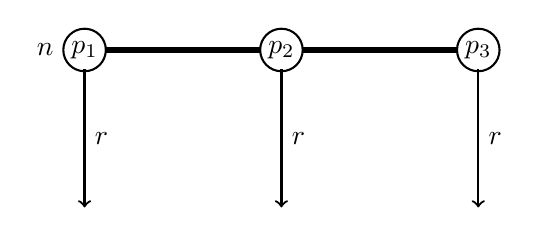
\begin{tikzpicture}

\begin{scope}[line width=2pt]
\draw (0,0) node at (-0.5,0) {$n$} -- (5,0);
\end{scope}

\begin{scope}[fill=white]
\filldraw  (0,0)  circle (2.7mm) node (nic) {$p_1$};
\filldraw  (2.5,0)  circle (2.7mm) node (nia) {$p_2$};
\filldraw  (5,0)  circle (2.7mm) node (nib) {$p_3$};
\end{scope}

\begin{scope}[thick,->]

\draw (nic) -- (0,-2) node [right, midway] {$r$};
\draw (nia) -- (2.5,-2) node [right, midway] {$r$};
\draw (nib) -- (5,-2) node [right, midway] {$r$};
\end{scope}

\end{tikzpicture}
\caption{A simple node $n$ with three processes $\{p_1, p_2, p_3\}$ in its domain, and the set of outcomes is $\{r\}$}
\label{fig:node}
\end{figure}

\subsubsection{A simple example: ATM workflow}
\label{example:ATM-untimed}

Before presenting a more elaborate scenario, we introduce negotiations through a simple example. Consider a transaction in an ATM machine ($a$), where a customer ($c$) wants to withdraw money from her bank ($b$).  Here, $a$, $c$, and $b$ are the \emph{processes} in the system. Their direct interactions are represented by thick horizontal lines (nodes). After each interaction, the participating agents decide on an outcome, represented by arrows. Initially, all agents are in the node $n_{in}$ node. They choose the outcome $st$ to start the transaction. Agents $a$ and $c$ go to node $n_1$ and $b$ goes to $n_2$.The customer gives her card details and requests for money withdrawal in the ATM at node $n_1$ by the outcome $req$. At $n_2$, the ATM conveys this request to the bank and sends the details through the outcome $det$. All three processes talk to each other at $n_3$, where the bank checks if there is sufficient money in the account and let the customer know via the ATM. They select $ok$ if the transaction is approved and go to $n_f$ otherwise they go back to $n_{in}$ by choosing the outcome $fail$.

\begin{figure}[t]
\centering
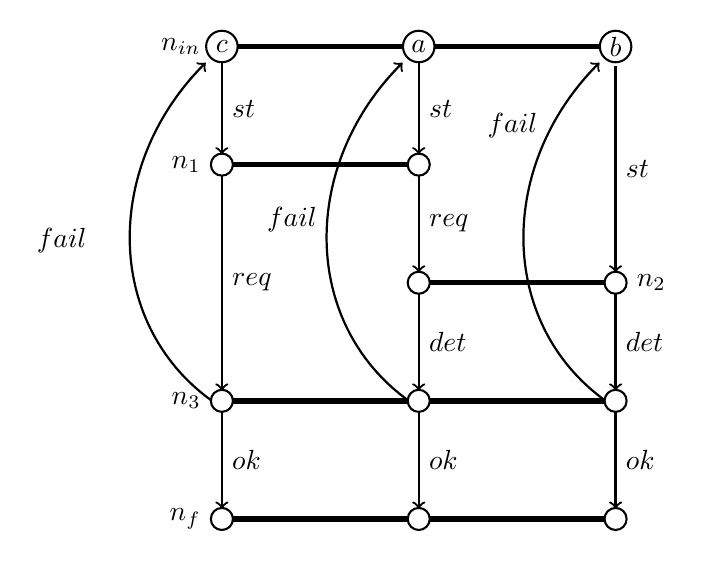
\begin{tikzpicture}

\begin{scope}[line width=2pt]
\draw (0.,0) node [left] {$n_{in}\,\,$} -- (5,0);
\draw (0.,-1.5) node [left] {$n_{1}\,\,$} -- (2.5,-1.5);
\draw (2.5,-3) -- (5,-3) node [right] {$\,\,n_{2}$};
\draw (0.,-4.5) node [left] {$n_{3}\,\,$} -- (5,-4.5);
\draw (0.,-6) node [left] {$n_{f}\,\,$} -- (5,-6);
\end{scope}

\begin{scope}[fill=white]
\filldraw  (0,0)  circle (2mm) node (nic) {$c$};
\filldraw  (2.5,0)  circle (2mm) node (nia) {$a$};
\filldraw  (5,0)  circle (2mm) node (nib) {$b$};

\filldraw  (0,-1.5)  circle (1.4mm) node (n1c) {};
\filldraw  (2.5,-1.5)  circle (1.4mm) node (n1a) {};

\filldraw  (2.5,-3)  circle (1.4mm) node (n2a) {};
\filldraw  (5,-3)  circle (1.4mm) node (n2b) {};

\filldraw  (0,-4.5)  circle (1.4mm) node (n3c) {};
\filldraw  (2.5,-4.5)  circle (1.4mm) node (n3a) {};
\filldraw  (5,-4.5)  circle (1.4mm) node (n3b) {};

\filldraw  (0,-6)  circle (1.4mm) node (n4c) {};
\filldraw  (2.5,-6)  circle (1.4mm) node (n4a) {};
\filldraw  (5,-6)  circle (1.4mm) node (n4b) {};
\end{scope}

\begin{scope}[thick,->]

\draw (nic) -- (n1c) node [right, midway] {$st$};
\draw (n1c) -- (n3c) node [right, midway] {$req$};
\draw (n3c) -- (n4c) node [right, midway] {$ok$};

\draw (nia) -- (n1a) node [right, midway] {$st$};
\draw (n1a) -- (n2a) node [right, midway] {$req$};
\draw (n2a) -- (n3a) node [right, midway] {$det$};
\draw (n3a) -- (n4a) node [right, midway] {$ok$};

\draw (nib) -- (n2b) node [right, midway] {$st$};
\draw (n2b) -- (n3b) node [right, midway] {$det$};
\draw (n3b) -- (n4b) node [right, midway] {$ok$};

\draw (n3c) + (-0.14,0.01) .. controls  (-1.5,-3.5) and (-1.5,-1.5) .. (nic) node [left=-0.2cm, text width = 1.25 cm, midway] {$fail$};
\draw (n3a) + (-0.14,0.01) .. controls  (1,-3.5) and (1,-1.5) .. (nia) node at (1.2,-2.2) [text width = 1.25 cm] {$fail$};
\draw (n3b) + (-0.14,0.01) .. controls  (3.5,-3.5) and (3.5,-1.5) .. (nib) node at (4,-1) [text width = 1.25 cm] {$fail$};

\end{scope}

\end{tikzpicture}
\caption{A distributed negotiations modelling a transaction between a customer, an ATM and a bank}
\label{fig:ATM}
\end{figure}


\begin{figure}[t]
\centering
\tikzset{every picture/.style={line width=0.75pt}} %set default line width to 0.75pt        

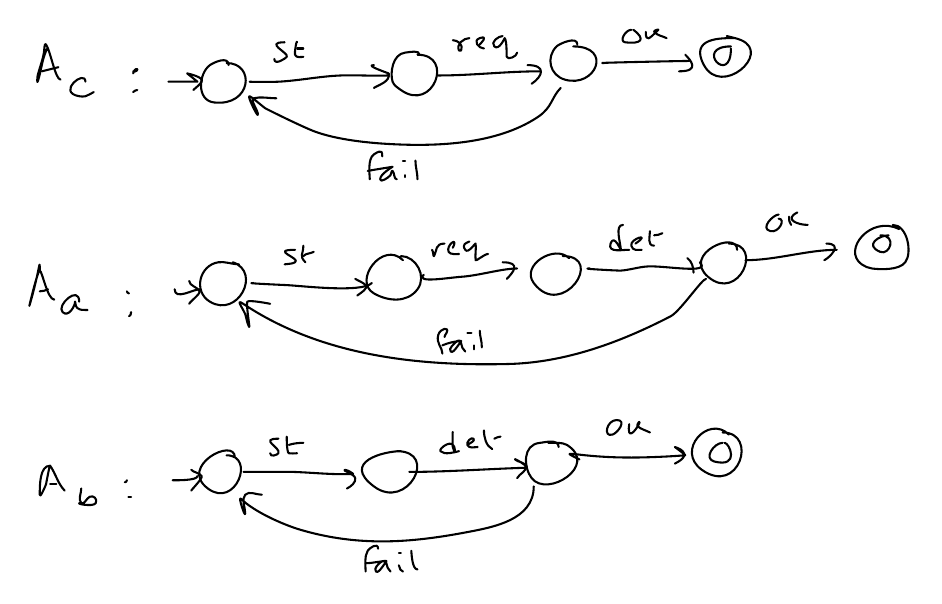
\begin{tikzpicture}[x=0.75pt,y=0.75pt,yscale=-1,xscale=1]
%uncomment if require: \path (0,300); %set diagram left start at 0, and has height of 300

%Shape: Free Drawing [id:dp699352073377679] 
\draw  [line width=0.75] [line join = round][line cap = round] (126,35) .. controls (126,30.35) and (118.72,33.77) .. (117,35) .. controls (111.56,38.89) and (110.28,52.03) .. (119,53) .. controls (137.12,55.01) and (139.04,34) .. (125,34) ;
%Shape: Free Drawing [id:dp20910792466845673] 
\draw  [line width=0.75] [line join = round][line cap = round] (218,30) .. controls (218,27.64) and (213.34,28.74) .. (211,29) .. controls (204.97,29.67) and (203.65,38.95) .. (205,43) .. controls (205.6,44.79) and (207.47,45.9) .. (209,47) .. controls (224.54,58.1) and (235.01,30) .. (217,30) ;
%Shape: Free Drawing [id:dp5846892232392498] 
\draw  [line width=0.75] [line join = round][line cap = round] (294,25) .. controls (294,20.83) and (285.31,24.69) .. (284,26) .. controls (278.68,31.32) and (280.76,39.93) .. (288,42) .. controls (302.83,46.24) and (311.37,26) .. (292,26) ;
%Shape: Free Drawing [id:dp6112448648060961] 
\draw  [line width=0.75] [line join = round][line cap = round] (370,22) .. controls (363.6,22) and (347.75,21.54) .. (355,35) .. controls (363.4,50.61) and (387.73,29.54) .. (373,23) .. controls (370.78,22.01) and (368.33,21.67) .. (366,21) ;
%Shape: Free Drawing [id:dp42021497143682085] 
\draw  [line width=0.75] [line join = round][line cap = round] (131,131) .. controls (127.65,131) and (124.31,129.49) .. (121,130) .. controls (111.93,131.4) and (108.77,144.06) .. (117,149) .. controls (130.47,157.08) and (142,134.67) .. (128,130) ;
%Shape: Free Drawing [id:dp9428654622094055] 
\draw  [line width=0.75] [line join = round][line cap = round] (210,129) .. controls (200.27,119.27) and (185.6,139.06) .. (196,145) .. controls (202.5,148.72) and (211.86,149.86) .. (217,143) .. controls (221.71,136.72) and (216.23,127) .. (209,127) ;
%Shape: Free Drawing [id:dp22523578617590523] 
\draw  [line width=0.75] [line join = round][line cap = round] (290,128) .. controls (283.18,121.18) and (266.55,131.4) .. (273,140) .. controls (286.56,158.09) and (307.8,127) .. (287,127) ;
%Shape: Free Drawing [id:dp6357001104153978] 
\draw  [line width=0.75] [line join = round][line cap = round] (371,124) .. controls (371,114.33) and (344.11,125.95) .. (357,137) .. controls (371.74,149.63) and (384.24,121) .. (367,121) ;
%Shape: Free Drawing [id:dp43290352630083795] 
\draw  [line width=0.75] [line join = round][line cap = round] (449,114) .. controls (435.4,107.2) and (421.33,124.09) .. (431,131) .. controls (432.46,132.04) and (434.22,132.76) .. (436,133) .. controls (439.62,133.48) and (449.01,133.98) .. (452,130) .. controls (455.53,125.3) and (452.98,112) .. (446,112) ;
%Shape: Free Drawing [id:dp4854772884625288] 
\draw  [line width=0.75] [line join = round][line cap = round] (129,224) .. controls (129,214.07) and (101.58,228.19) .. (116,239) .. controls (129.38,249.03) and (139.18,223) .. (125,223) ;
%Shape: Free Drawing [id:dp3971045256545481] 
\draw  [line width=0.75] [line join = round][line cap = round] (209,221) .. controls (200.93,221) and (180.13,226.1) .. (196,238) .. controls (212.1,250.07) and (227.59,221) .. (207,221) ;
%Shape: Free Drawing [id:dp4509421284855678] 
\draw  [line width=0.75] [line join = round][line cap = round] (285,219) .. controls (285,214.88) and (278.13,216.81) .. (276,217) .. controls (267.43,217.78) and (268.11,229) .. (272,234) .. controls (279.6,243.78) and (304.55,227.72) .. (289,218) .. controls (286.75,216.6) and (282.29,217) .. (280,217) ;
%Shape: Free Drawing [id:dp24931842316411212] 
\draw  [line width=0.75] [line join = round][line cap = round] (367,213) .. controls (357.27,203.27) and (341.05,220.75) .. (354,230) .. controls (371.89,242.78) and (381.31,212) .. (364,212) ;
%Shape: Free Drawing [id:dp9658349676228442] 
\draw  [line width=0.75] [line join = round][line cap = round] (39,27) .. controls (39,25.51) and (37.42,29.57) .. (37,31) .. controls (35.84,34.96) and (35.3,39.09) .. (34,43) .. controls (33.68,43.95) and (33.76,40.97) .. (34,40) .. controls (34.97,36.11) and (36.35,32.93) .. (37,29) .. controls (37.23,27.64) and (37.24,23.86) .. (38,25) .. controls (40.19,28.28) and (42.53,42) .. (45,42) ;
%Shape: Free Drawing [id:dp09004794014509787] 
\draw  [line width=0.75] [line join = round][line cap = round] (36,38) .. controls (38.67,37.33) and (41.33,36.67) .. (44,36) ;
%Shape: Free Drawing [id:dp6821526471402938] 
\draw  [line width=0.75] [line join = round][line cap = round] (57,43) .. controls (57,36.82) and (42.78,48.13) .. (54,50) .. controls (54.99,50.16) and (56.04,50.27) .. (57,50) .. controls (58.43,49.59) and (59.67,48.67) .. (61,48) ;
%Shape: Free Drawing [id:dp19914947748820078] 
\draw  [line width=0.75] [line join = round][line cap = round] (80,38) .. controls (80,38.75) and (82.53,37.53) .. (82,37) .. controls (81.33,36.33) and (80,38.06) .. (80,39) ;
%Shape: Free Drawing [id:dp22950086205936715] 
\draw  [line width=0.75] [line join = round][line cap = round] (80,48) .. controls (80.53,47.47) and (81.25,47) .. (82,47) ;
%Shape: Free Drawing [id:dp8458179935856099] 
\draw  [line width=0.75] [line join = round][line cap = round] (35,134) .. controls (35,126.72) and (35.09,133.7) .. (30,151) .. controls (29.68,152.08) and (33.95,134) .. (35,134) .. controls (36.12,134) and (38.71,148) .. (42,148) ;
%Shape: Free Drawing [id:dp8709509858246236] 
\draw  [line width=0.75] [line join = round][line cap = round] (35,144) .. controls (36.37,144) and (37.77,143.61) .. (39,143) ;
%Shape: Free Drawing [id:dp1689306225658136] 
\draw  [line width=0.75] [line join = round][line cap = round] (54,149) .. controls (54,140.69) and (42.78,150.78) .. (46,154) .. controls (48.77,156.77) and (52,151.14) .. (52,149) .. controls (52,147.95) and (52.16,151.37) .. (53,152) .. controls (54.61,153.21) and (56.22,153) .. (58,153) ;
%Shape: Free Drawing [id:dp9154214496730456] 
\draw  [line width=0.75] [line join = round][line cap = round] (77,144) .. controls (77,144.47) and (77.53,145) .. (78,145) ;
%Shape: Free Drawing [id:dp0780602300217802] 
\draw  [line width=0.75] [line join = round][line cap = round] (78,156) .. controls (78.75,156) and (79,154.75) .. (79,154) ;
%Shape: Free Drawing [id:dp8104400124521838] 
\draw  [line width=0.75] [line join = round][line cap = round] (40,228) .. controls (35.04,228) and (35,237.04) .. (35,242) .. controls (35,243.94) and (37.32,238.82) .. (38,237) .. controls (38.1,236.73) and (39.71,227.58) .. (40,228) .. controls (42.66,231.79) and (43.73,236.73) .. (47,240) ;
%Shape: Free Drawing [id:dp1836175709335458] 
\draw  [line width=0.75] [line join = round][line cap = round] (40,237) .. controls (41,237) and (42,237) .. (43,237) ;
%Shape: Free Drawing [id:dp5761019515015455] 
\draw  [line width=0.75] [line join = round][line cap = round] (55,239) .. controls (55,241.33) and (53.35,244.35) .. (55,246) .. controls (56.18,247.18) and (57.51,243.75) .. (59,243) .. controls (60.91,242.05) and (62.95,244.09) .. (62,246) .. controls (60.9,248.19) and (50.6,246) .. (55,246) ;
%Shape: Free Drawing [id:dp11510509263160207] 
\draw  [line width=0.75] [line join = round][line cap = round] (76,236) .. controls (76.47,236) and (77,235.47) .. (77,235) ;
%Shape: Free Drawing [id:dp1326029043307244] 
\draw  [line width=0.75] [line join = round][line cap = round] (78,243) .. controls (76.79,243) and (77.96,243) .. (79,243) ;
%Shape: Free Drawing [id:dp47687509882848156] 
\draw  [line width=0.75] [line join = round][line cap = round] (100,43) .. controls (88.71,43) and (111,43) .. (111,43) .. controls (111,43) and (106,39) .. (106,39) .. controls (106,39) and (114.38,40.7) .. (113,43) .. controls (112.03,44.62) and (110.33,45.67) .. (109,47) ;
%Shape: Free Drawing [id:dp2442975775805618] 
\draw  [line width=0.75] [line join = round][line cap = round] (100,143) .. controls (100,148.52) and (108.95,143) .. (112,143) ;
%Shape: Free Drawing [id:dp3598381417417724] 
\draw  [line width=0.75] [line join = round][line cap = round] (107,139) .. controls (107,141.36) and (111.07,141.83) .. (112,144) .. controls (112.49,145.15) and (107.59,148.82) .. (107,150) ;
%Shape: Free Drawing [id:dp7335814100329172] 
\draw  [line width=0.75] [line join = round][line cap = round] (99,235) .. controls (99.04,235) and (111,235.38) .. (111,233) ;
%Shape: Free Drawing [id:dp3988930161980966] 
\draw  [line width=0.75] [line join = round][line cap = round] (108,230) .. controls (109.37,231.37) and (111.92,231.38) .. (113,233) .. controls (113.63,233.95) and (108.75,238.88) .. (108,240) ;
%Shape: Free Drawing [id:dp5504071776051671] 
\draw  [line width=0.75] [line join = round][line cap = round] (137,43) .. controls (132.67,43) and (145.67,43.23) .. (150,43) .. controls (159.94,42.48) and (170.09,40.37) .. (180,40) .. controls (187.66,39.72) and (195.34,40.33) .. (203,40) .. controls (203.33,39.99) and (203.33,39) .. (203,39) ;
%Shape: Free Drawing [id:dp38092617558048913] 
\draw  [line width=0.75] [line join = round][line cap = round] (196,35) .. controls (191.21,35) and (202.94,38.83) .. (203,39) .. controls (204.31,42.93) and (197.91,44.64) .. (196,46) ;
%Shape: Free Drawing [id:dp3455480331109182] 
\draw  [line width=0.75] [line join = round][line cap = round] (227,40) .. controls (243.44,40) and (259.78,38) .. (276,38) ;
%Shape: Free Drawing [id:dp0471808156338025] 
\draw  [line width=0.75] [line join = round][line cap = round] (270,35) .. controls (279.42,35) and (277.22,40.52) .. (272,44) ;
%Shape: Free Drawing [id:dp03599926708867218] 
\draw  [line width=0.75] [line join = round][line cap = round] (307,34) .. controls (298.31,34) and (343.84,33) .. (348,33) ;
%Shape: Free Drawing [id:dp60137065125319] 
\draw  [line width=0.75] [line join = round][line cap = round] (346,30) .. controls (348.43,32.43) and (353.55,38) .. (343,38) ;
%Shape: Free Drawing [id:dp6317644494836507] 
\draw  [line width=0.75] [line join = round][line cap = round] (286,46) .. controls (281.46,50.54) and (281.99,55.34) .. (275,60) .. controls (255.09,73.27) and (226.16,74.32) .. (203,73) .. controls (191.49,72.34) and (175.52,70.6) .. (165,66) .. controls (157.9,62.89) and (150.93,59.47) .. (144,56) .. controls (142.76,55.38) and (136.92,50) .. (136,50) .. controls (134.93,50) and (139.75,59.5) .. (140,59) .. controls (140.75,57.5) and (136,51.55) .. (138,51) .. controls (141.54,50.04) and (145.33,51) .. (149,51) ;
%Shape: Free Drawing [id:dp5041132373888955] 
\draw  [line width=0.75] [line join = round][line cap = round] (153,24) .. controls (142.74,24) and (155.35,29.2) .. (154,31) .. controls (153.34,31.88) and (148,35.38) .. (148,32) ;
%Shape: Free Drawing [id:dp9052641536236868] 
\draw  [line width=0.75] [line join = round][line cap = round] (159,24) .. controls (159,21.97) and (157.67,28) .. (158,30) .. controls (158.28,31.71) and (161.55,31) .. (162,31) ;
%Shape: Free Drawing [id:dp00037039861442378363] 
\draw  [line width=0.75] [line join = round][line cap = round] (159,27) .. controls (160,27) and (161,27) .. (162,27) ;
%Shape: Free Drawing [id:dp3222100625858557] 
\draw  [line width=0.75] [line join = round][line cap = round] (234,23) .. controls (236.36,23) and (239.38,25.24) .. (238,28) .. controls (237.85,28.3) and (237.15,28.3) .. (237,28) .. controls (235.48,24.97) and (239.25,22) .. (242,22) ;
%Shape: Free Drawing [id:dp8528288775510539] 
\draw  [line width=0.75] [line join = round][line cap = round] (247,25) .. controls (247.37,24.63) and (251.6,20.47) .. (247,22) .. controls (243.41,23.2) and (246.47,27) .. (249,27) ;
%Shape: Free Drawing [id:dp6245891639619918] 
\draw  [line width=0.75] [line join = round][line cap = round] (258,21) .. controls (256.1,21) and (251.91,23.91) .. (254,26) .. controls (256.19,28.19) and (259,22) .. (259,22) .. controls (260.08,23.08) and (259.88,30.4) .. (260,31) .. controls (260.35,32.76) and (265,30.8) .. (265,29) ;
%Shape: Free Drawing [id:dp2955298345225923] 
\draw  [line width=0.75] [line join = round][line cap = round] (320,18) .. controls (317.07,18) and (314.05,23.63) .. (317,24) .. controls (324.7,24.96) and (327.28,22.71) .. (321,18) ;
%Shape: Free Drawing [id:dp7650219261943041] 
\draw  [line width=0.75] [line join = round][line cap = round] (327,19) .. controls (327,24.19) and (328.59,22.41) .. (333,18) .. controls (333.53,17.47) and (330.47,18.47) .. (331,19) .. controls (333.05,21.05) and (334.69,20.84) .. (337,22) ;
%Shape: Free Drawing [id:dp9858048471107251] 
\draw  [line width=0.75] [line join = round][line cap = round] (200,79) .. controls (200,77.39) and (200.33,75.11) .. (196,78) .. controls (192.81,80.13) and (194,88.12) .. (194,90) ;
%Shape: Free Drawing [id:dp27682562555764234] 
\draw  [line width=0.75] [line join = round][line cap = round] (193,86) .. controls (194.11,85.72) and (205,84) .. (205,84) .. controls (205,84) and (199,87.47) .. (199,90) .. controls (199,91.8) and (202.88,89.4) .. (204,88) .. controls (204.47,87.42) and (204.47,85.47) .. (205,86) .. controls (206.05,87.05) and (205.51,90) .. (207,90) ;
%Shape: Free Drawing [id:dp9843351866594481] 
\draw  [line width=0.75] [line join = round][line cap = round] (211,88) .. controls (211,88.33) and (211,88.67) .. (211,89) ;
%Shape: Free Drawing [id:dp7139829189684593] 
\draw  [line width=0.75] [line join = round][line cap = round] (211,81) .. controls (209.67,81) and (209.67,81) .. (211,81) ;
%Shape: Free Drawing [id:dp9021117212192773] 
\draw  [line width=0.75] [line join = round][line cap = round] (216,81) .. controls (216,84.02) and (217,86.98) .. (217,90) ;
%Shape: Free Drawing [id:dp44700280018755034] 
\draw  [line width=0.75] [line join = round][line cap = round] (368,26) .. controls (349.6,26) and (368,45.62) .. (368,27) ;
%Shape: Free Drawing [id:dp36075313476514703] 
\draw  [line width=0.75] [line join = round][line cap = round] (138,140) .. controls (132.66,140) and (148.66,140.76) .. (154,141) .. controls (160.98,141.32) and (190.11,144.89) .. (195,140) ;
%Shape: Free Drawing [id:dp6900079518028266] 
\draw  [line width=0.75] [line join = round][line cap = round] (187,138) .. controls (188.67,139) and (190.63,139.63) .. (192,141) .. controls (193.51,142.51) and (189.71,144.72) .. (188,146) ;
%Shape: Free Drawing [id:dp857009029163824] 
\draw  [line width=0.75] [line join = round][line cap = round] (220,136) .. controls (215.75,140.25) and (232,137.4) .. (238,137) .. controls (246.64,136.42) and (257.64,133) .. (265,133) ;
%Shape: Free Drawing [id:dp7791873524744648] 
\draw  [line width=0.75] [line join = round][line cap = round] (258,130) .. controls (267.22,130) and (263.14,134.86) .. (260,138) ;
%Shape: Free Drawing [id:dp030091329506495068] 
\draw  [line width=0.75] [line join = round][line cap = round] (300,133) .. controls (293.94,133) and (313.66,134.09) .. (315,134) .. controls (319.37,133.7) and (323.62,132.22) .. (328,132) .. controls (336.35,131.57) and (358.91,135.91) .. (353,130) ;
%Shape: Free Drawing [id:dp6794109558694876] 
\draw  [line width=0.75] [line join = round][line cap = round] (347,128) .. controls (349.11,129.41) and (350,132.46) .. (350,135) ;
%Shape: Free Drawing [id:dp4941635414386235] 
\draw  [line width=0.75] [line join = round][line cap = round] (158,124) .. controls (145.53,124) and (161.16,128.1) .. (158,130) .. controls (156.54,130.87) and (154.67,130.67) .. (153,131) ;
%Shape: Free Drawing [id:dp08363776027723879] 
\draw  [line width=0.75] [line join = round][line cap = round] (162,122) .. controls (162,126.3) and (159.8,126.8) .. (163,130) ;
%Shape: Free Drawing [id:dp17133608241358922] 
\draw  [line width=0.75] [line join = round][line cap = round] (162,127) .. controls (163.43,125.57) and (165.08,125.96) .. (167,125) ;
%Shape: Free Drawing [id:dp42444576991187455] 
\draw  [line width=0.75] [line join = round][line cap = round] (224,124) .. controls (224.75,124.75) and (224.53,127.94) .. (225,127) .. controls (226.45,124.11) and (225.48,121) .. (230,121) ;
%Shape: Free Drawing [id:dp42354377365438856] 
\draw  [line width=0.75] [line join = round][line cap = round] (234,123) .. controls (236.99,117.03) and (230.46,121.93) .. (232,125) .. controls (232.72,126.45) and (236.17,126) .. (237,126) ;
%Shape: Free Drawing [id:dp254637723356695] 
\draw  [line width=0.75] [line join = round][line cap = round] (242,120) .. controls (240.5,120.75) and (238.13,121.19) .. (240,124) .. controls (241.41,126.12) and (244.93,120.44) .. (245,121) .. controls (245.33,123.65) and (244.67,126.35) .. (245,129) .. controls (245.09,129.7) and (249.25,126) .. (251,126) ;
%Shape: Free Drawing [id:dp8660053496027834] 
\draw  [line width=0.75] [line join = round][line cap = round] (316,112) .. controls (311.99,112) and (314.67,120) .. (315,124) .. controls (315.06,124.76) and (311.71,115.88) .. (310,121) .. controls (308.39,125.84) and (316.64,123.74) .. (319,124) ;
%Shape: Free Drawing [id:dp5631701100684178] 
\draw  [line width=0.75] [line join = round][line cap = round] (322,121) .. controls (330.22,115.52) and (319.15,118.59) .. (320,122) .. controls (320.68,124.71) and (323.21,124) .. (325,124) ;
%Shape: Free Drawing [id:dp05369272016552906] 
\draw  [line width=0.75] [line join = round][line cap = round] (329,115) .. controls (329,117.48) and (327.44,122) .. (331,122) ;
%Shape: Free Drawing [id:dp7255991302691805] 
\draw  [line width=0.75] [line join = round][line cap = round] (331,117) .. controls (332.37,117) and (333.77,116.61) .. (335,116) ;
%Shape: Free Drawing [id:dp26821501258625524] 
\draw  [line width=0.75] [line join = round][line cap = round] (375,129) .. controls (389.77,129) and (404.91,124) .. (419,124) ;
%Shape: Free Drawing [id:dp19135576727743342] 
\draw  [line width=0.75] [line join = round][line cap = round] (414,121) .. controls (422.3,121) and (415.75,127.63) .. (413,129) ;
%Shape: Free Drawing [id:dp9970516135074035] 
\draw  [line width=0.75] [line join = round][line cap = round] (391,107) .. controls (388.45,107) and (381.8,113.7) .. (387,115) .. controls (391.11,116.03) and (394.61,109) .. (391,109) ;
%Shape: Free Drawing [id:dp7586304194815168] 
\draw  [line width=0.75] [line join = round][line cap = round] (396,108) .. controls (396,109.37) and (396.03,111.03) .. (397,112) ;
%Shape: Free Drawing [id:dp011025846487307756] 
\draw  [line width=0.75] [line join = round][line cap = round] (400,106) .. controls (393.21,109.39) and (400.38,112) .. (405,112) ;
%Shape: Free Drawing [id:dp19856863207902364] 
\draw  [line width=0.75] [line join = round][line cap = round] (444,117) .. controls (439.43,117) and (431.97,121.79) .. (440,125) .. controls (444.48,126.79) and (448.25,117) .. (440,117) ;
%Shape: Free Drawing [id:dp8137485876937424] 
\draw  [line width=0.75] [line join = round][line cap = round] (356,138) .. controls (354.11,138) and (343.46,153.69) .. (339,156) .. controls (314.76,168.54) and (288.51,178.29) .. (261,179) .. controls (216.71,180.14) and (170.45,174.97) .. (133,150) .. controls (129.25,147.5) and (132.38,151.36) .. (134,155) .. controls (134.56,156.26) and (134.49,157.72) .. (135,159) .. controls (135.28,159.69) and (136,161.75) .. (136,161) .. controls (136,160.05) and (134.32,149.68) .. (135,149) .. controls (136,148) and (145.68,149.95) .. (146,150) ;
%Shape: Free Drawing [id:dp670488850721851] 
\draw  [line width=0.75] [line join = round][line cap = round] (230,166) .. controls (230,165.25) and (230.67,164.67) .. (231,164) .. controls (232.62,160.77) and (227.92,161.78) .. (227,165) .. controls (225.8,169.21) and (229,170.78) .. (229,174) ;
%Shape: Free Drawing [id:dp3729587461127226] 
\draw  [line width=0.75] [line join = round][line cap = round] (229,170) .. controls (231.85,168.86) and (234.93,168) .. (238,168) .. controls (238.67,168) and (236.47,167.53) .. (236,168) .. controls (234.63,169.37) and (231.63,171.63) .. (233,173) .. controls (234.51,174.51) and (238,166.87) .. (238,169) .. controls (238,170.49) and (238.95,171.95) .. (240,173) ;
%Shape: Free Drawing [id:dp5973208170734658] 
\draw  [line width=0.75] [line join = round][line cap = round] (244,170) .. controls (244,170.67) and (244,171.33) .. (244,172) ;
%Shape: Free Drawing [id:dp6273152642236075] 
\draw  [line width=0.75] [line join = round][line cap = round] (241,164) .. controls (241.67,164) and (242.33,164) .. (243,164) ;
%Shape: Free Drawing [id:dp2664250327058062] 
\draw  [line width=0.75] [line join = round][line cap = round] (247,163) .. controls (247,165.89) and (248,167.48) .. (248,171) ;
%Shape: Free Drawing [id:dp09767215156309195] 
\draw  [line width=0.75] [line join = round][line cap = round] (135,231) .. controls (125.32,231) and (157,231) .. (157,231) .. controls (166.67,231.32) and (176.34,232.44) .. (186,232) .. controls (186.33,231.98) and (183.28,230) .. (182,230) .. controls (179.87,230) and (186.58,231.91) .. (187,234) .. controls (187.42,236.09) and (184.91,238.05) .. (183,239) ;
%Shape: Free Drawing [id:dp4557189487035944] 
\draw  [line width=0.75] [line join = round][line cap = round] (213,231) .. controls (231.28,231) and (250.84,229.57) .. (269,229) .. controls (271.63,228.92) and (262.95,223.95) .. (264,225) .. controls (265.37,226.37) and (268.39,226.16) .. (269,228) .. controls (269.96,230.87) and (266.19,231.63) .. (265,234) ;
%Shape: Free Drawing [id:dp04523814859365094] 
\draw  [line width=0.75] [line join = round][line cap = round] (295,225) .. controls (283.05,219.03) and (293.86,224.8) .. (326,224) .. controls (332.67,223.83) and (339.34,223.51) .. (346,223) .. controls (346.37,222.97) and (341,219) .. (341,219) .. controls (341,219) and (351.22,221.89) .. (341,227) ;
%Shape: Free Drawing [id:dp43397584755084206] 
\draw  [line width=0.75] [line join = round][line cap = round] (150,215) .. controls (140.29,215) and (151.32,219.35) .. (150,222) .. controls (149.69,222.62) and (146,224.29) .. (146,222) ;
%Shape: Free Drawing [id:dp7766950236050176] 
\draw  [line width=0.75] [line join = round][line cap = round] (154,215) .. controls (154,210.61) and (153.76,221.69) .. (155,222) .. controls (156.29,222.32) and (157.67,222) .. (159,222) ;
%Shape: Free Drawing [id:dp8010900191079826] 
\draw  [line width=0.75] [line join = round][line cap = round] (155,218) .. controls (157.24,217.25) and (159.64,217) .. (162,217) ;
%Shape: Free Drawing [id:dp3926412888334434] 
\draw  [line width=0.75] [line join = round][line cap = round] (234,212) .. controls (234,209.67) and (233.77,216.68) .. (234,219) .. controls (234.07,219.74) and (235,221.75) .. (235,221) .. controls (235,213.4) and (226.94,219.94) .. (228,221) .. controls (230,223) and (234.87,221.53) .. (237,221) ;
%Shape: Free Drawing [id:dp1463435029012543] 
\draw  [line width=0.75] [line join = round][line cap = round] (241,218) .. controls (242.18,217.22) and (245,216) .. (244,215) .. controls (242.98,213.98) and (240.33,216.67) .. (241,218) .. controls (241.97,219.94) and (244.28,219) .. (246,219) ;
%Shape: Free Drawing [id:dp14438813709444898] 
\draw  [line width=0.75] [line join = round][line cap = round] (249,211) .. controls (249,214.28) and (250.06,218.53) .. (253,220) ;
%Shape: Free Drawing [id:dp6870409972621128] 
\draw  [line width=0.75] [line join = round][line cap = round] (254,215) .. controls (254.94,214.53) and (255.95,214) .. (257,214) ;
%Shape: Free Drawing [id:dp6342421719103655] 
\draw  [line width=0.75] [line join = round][line cap = round] (313,206) .. controls (308.03,206) and (306.28,214.57) .. (311,213) .. controls (313.49,212.17) and (318.07,206) .. (313,206) -- cycle ;
%Shape: Free Drawing [id:dp46663802286189726] 
\draw  [line width=0.75] [line join = round][line cap = round] (319,208) .. controls (319,209.33) and (318.4,210.81) .. (319,212) .. controls (320.13,214.27) and (324,207.98) .. (324,207) .. controls (324,206.25) and (322.43,208.52) .. (323,209) .. controls (324.72,210.43) and (327,211) .. (329,212) ;
%Shape: Free Drawing [id:dp21435444815750926] 
\draw  [line width=0.75] [line join = round][line cap = round] (273,238) .. controls (273,254.24) and (253.22,257.67) .. (241,260) .. controls (213.34,265.27) and (188.57,267) .. (161,259) .. controls (151.75,256.32) and (137.84,249.84) .. (132,244) .. controls (130.28,242.28) and (134,253.43) .. (134,251) .. controls (134,248) and (132.01,244.24) .. (134,242) .. controls (135.77,240.01) and (139.33,242) .. (142,242) ;
%Shape: Free Drawing [id:dp49544639169575677] 
\draw  [line width=0.75] [line join = round][line cap = round] (198,268) .. controls (198,264.62) and (193.72,267.79) .. (193,269) .. controls (191.26,271.9) and (192,276.08) .. (192,279) ;
%Shape: Free Drawing [id:dp7435150702646659] 
\draw  [line width=0.75] [line join = round][line cap = round] (192,275) .. controls (195.57,275) and (198.37,274) .. (202,274) .. controls (202.67,274) and (200.57,273.66) .. (200,274) .. controls (198.33,275) and (195.63,277.63) .. (197,279) .. controls (198.51,280.51) and (202,272.87) .. (202,275) .. controls (202,276.49) and (202.95,277.95) .. (204,279) ;
%Shape: Free Drawing [id:dp14850568602306735] 
\draw  [line width=0.75] [line join = round][line cap = round] (208,276) .. controls (208.75,277.51) and (208.55,279) .. (210,279) ;
%Shape: Free Drawing [id:dp44143806738856406] 
\draw  [line width=0.75] [line join = round][line cap = round] (208,270) .. controls (208.33,270) and (208.67,270) .. (209,270) ;
%Shape: Free Drawing [id:dp9803674578133618] 
\draw  [line width=0.75] [line join = round][line cap = round] (214,269) .. controls (214.12,269.82) and (214.31,278) .. (217,278) ;
%Shape: Free Drawing [id:dp5266452546165475] 
\draw  [line width=0.75] [line join = round][line cap = round] (364,217) .. controls (359.78,217) and (354.58,224.64) .. (360,226) .. controls (372.61,229.15) and (367.22,217) .. (365,217) ;




\end{tikzpicture}
\caption{A network of automata over distributed alphabet negotiation modelling the same transaction}
\label{fig:ATM}
\end{figure}

\subsubsection{Semantics}
To reason about reachability, however, we require a precise notion of system evolution. We therefore briefly recall the operational semantics of negotiations. A \emph{marking} describes, for each process, the set of nodes at which it is currently ready to participate. Graphically, a marking is represented by placing tokens (black dots) on the forking points of hyperarcs (or on the arcs themselves when there is no branching). A node \(n\) is \emph{enabled} in a marking \(x\) if all processes in the domain of \(n\) are currently ready to engage in \(n\). When \(n\) is enabled, the agents at \(n\) jointly choose an outcome \(r\); we say that the \emph{outcome} \((n,r)\) \emph{occurs}. This yields a new marking \(x'\), written
\[
x \xrightarrow{(n,r)} x'.
\]
Such a step is called a \emph{small step}. A \emph{run} of a negotiation is a (finite or infinite) sequence of small steps
\[
x_0 \xrightarrow{(n_1,r_1)} x_1 \xrightarrow{(n_2,r_2)} x_2 \cdots
\]
and the corresponding word \(\sigma = (n_1,r_1)(n_2,r_2)\dots\) is called an \emph{occurrence sequence}. A marking that enables no node is called a \emph{deadlock}. A marking from which the final marking is unreachable, yet which can reoccur along some run, is called a \emph{livelock}.

Having introduced the basic concepts through this simple workflow, we now turn to a more complex example that demonstrates richer branching and outcome dependencies.

\subsubsection{A more complex example: Pollination and climate change}
\label{subsubsec:pollination-example}

We now consider a more elaborate negotiation inspired by ecological phenomena. This example is not intended as a faithful ecological model, but as a stylized concurrent system exhibiting partial synchronization and branching. 

The early flowering of many plants due to climate change creates critical synchronization challenges for insect pollinators such as bees. Figure~\ref{fig:pollination} presents an illustrative example adapted from an ecological scenario that demonstrates an incomplete negotiation. The system comprises three processes: \(t\) (trees), \(e\) (environment), and \(b\) (bees). Nodes represent negotiation points corresponding to events such as seasonal changes, climate conditions, and flowering behavior, while outcomes represent qualitative results including ``good climate'', ``climate change'', ``normal flowering'', and ``early flowering''.

In Figure~\ref{fig:pollitation}, node $n_4$ involves two processes, $t$ and $e$, which participate in the negotiation (depicted as ports in the figure). We refer to the set of participating processes as the domain of the node; thus, the domain of $n_4$ is $\{t, e\}$. In contrast, node $n_3$ has only process $b$ in its domain. Each node features outgoing actions in which all processes within that node's domain must participate collectively. For instance, $n_6$ has a single outgoing action $nl$, while $n_2$ has two outgoing actions, $gc$ and $ch$.

The diagram uses hyperarcs to denote non-deterministic outgoing edges, as seen with actions $sc$ and $e$. When action $sc$ is taken from $n_1$, process $t$ becomes ready to engage with both nodes $n_4$ and $n_5$. Non-hyperarcs represent deterministic edges. 

\begin{figure}[t]
\centering
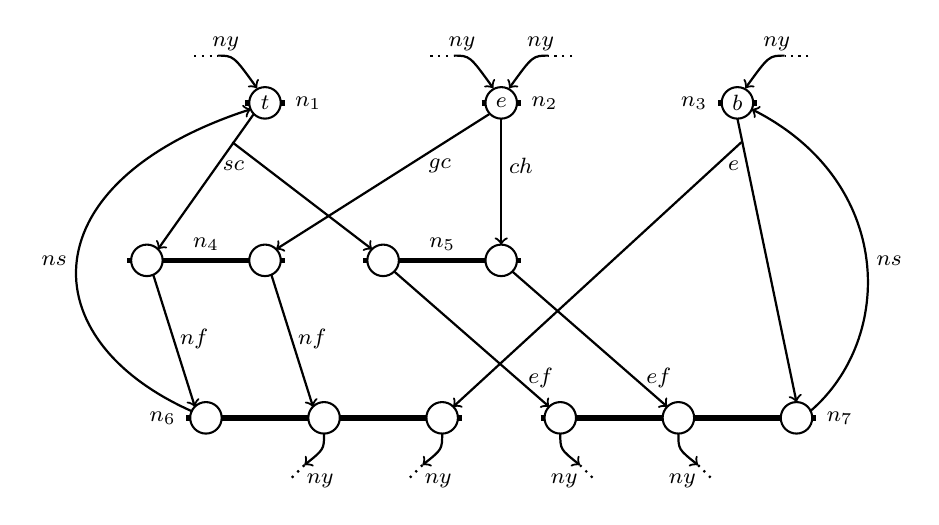
\begin{tikzpicture}[scale=1, every node/.style={transform shape}]

\begin{scope}[line width=2pt]
\draw (-0.25,0) -- (0.25,0);
\draw (2.75,0) -- (3.25,0);
\draw (5.75,0) -- (6.25,0);
\draw (-1.75,-2) -- (0.25,-2);
\draw (1.25,-2) -- (3.25,-2);
\draw (-1,-4) -- (2.5,-4);
\draw (3.5,-4) -- (7,-4);
\end{scope}

\filldraw [fill=white]  (0,0)  circle (2mm) node (t0) {\footnotesize $t$};
\filldraw [fill=white]  (3,0)  circle (2mm) node (e0) {\footnotesize $e$};
\filldraw [fill=white]  (6,0)  circle (2mm) node (b0) {\footnotesize $b$};
\filldraw [fill=white]  (-1.5,-2)  circle (2mm) node (t1) {};
\filldraw [fill=white]  (0,-2)  circle (2mm) node (e1) {};
\filldraw [fill=white]  (1.5,-2)  circle (2mm) node (t2) {};
\filldraw [fill=white]  (3,-2)  circle (2mm) node (e2) {};
\filldraw [fill=white]  (-0.75,-4)  circle (2mm) node (t5) {};
\filldraw [fill=white]  (0.75,-4)  circle (2mm) node (e5) {};
\filldraw [fill=white]  (2.25,-4)  circle (2mm) node (b5) {};
\filldraw [fill=white]  (3.75,-4)  circle (2mm) node (t6) {};
\filldraw [fill=white]  (5.25,-4)  circle (2mm) node (e6) {};
\filldraw [fill=white]  (6.75,-4)  circle (2mm) node (b6) {};

\node at (0.55,0) {\footnotesize $n_1$};
\node at (3.55,0) {\footnotesize $n_2$};
\node at (5.45,0) {\footnotesize $n_3$};
\node at (-0.75,-1.8) {\footnotesize $n_4$};
\node at (2.25,-1.8) {\footnotesize $n_5$};
\node at (-1.3,-4) {\footnotesize $n_6$};
\node at (7.3,-4) {\footnotesize $n_7$};

\node at (-0.4, -0.8) {\footnotesize $sc$};
\node at (2.22, -0.8) {\footnotesize $gc$};
\node at (3.25, -0.8) {\footnotesize $ch$};
\node at (5.95, -0.8) {\footnotesize $e$};
\node at (-0.9,-3) {\footnotesize $nf$};
\node at (0.6, -3) {\footnotesize $nf$};
\node at (3.5,-3.5) {\footnotesize $ef$};
\node at (5,-3.5) {\footnotesize $ef$};
\node at (0.7, -4.8) {\footnotesize $ny$};
\node at (2.2, -4.8) {\footnotesize $ny$};
\node at (3.8, -4.8) {\footnotesize $ny$};
\node at (5.3, -4.8) {\footnotesize $ny$};
\node at (-0.5, 0.75) {\footnotesize $ny$};
\node at (2.5, 0.75) {\footnotesize $ny$};
\node at (3.5, 0.75) {\footnotesize $ny$};
\node at (6.5, 0.75) {\footnotesize $ny$};

\begin{scope}[thick,->]
\draw (-0.145, -0.145) -- (-1.36, -1.86); % t0-t1
\draw (-0.415, -0.5) -- (1.36, -1.86); % t0-t2
\draw (2.845, -0.145) -- (0.14, -1.86); % e0-e1
\draw (3, -0.2) -- (3, -1.8); % e0-e2
\draw (-1.5, -2) + (0.08, -0.18) -- (-0.89, -3.86); % t1-t3
\draw (0, -2) + (0.08, -0.18) -- (0.61, -3.86); % e1-e3
\draw (1.5, -2) + (0.145, -0.145) -- (3.61, -3.86); % t2-t4
\draw (3, -2) + (0.145, -0.145) -- (5.11, -3.86); % e2-e4
\draw (6.05, -0.5) -- (2.39, -3.86); % b0-b3
\draw (6, -0.2) -- (6.75, -3.8); % b0-b4
\draw (-0.92, -3.92) .. controls (-3, -3) and (-3, -1) .. (-0.18, -0.08) node [midway, left] {\footnotesize $ns$}; % t3-t0
\draw (6.92, -3.92) .. controls (8, -3) and (8, -1) .. (6.18, -0.08) node [midway, right] {\footnotesize $ns$}; % b4-b0
\draw (0.75,-4.2) .. controls (0.75, -4.4) .. (0.5,-4.6); % e3-e0
\draw (2.25, -4.2) .. controls (2.25, -4.4) .. (2, -4.6); % b3-b0
\draw (3.75, -4.2) .. controls (3.75, -4.4) .. (4, -4.6); % t4-t0
\draw (5.25, -4.2) .. controls (5.25, -4.4) .. (5.5, -4.6); % e4-e0
\draw (-0.6, 0.6) .. controls (-0.4, 0.6) .. (-0.1, 0.185); % t4-t0
\draw (2.4, 0.6) .. controls (2.6, 0.6) .. (2.9, 0.185); % e3-e0
\draw (3.6, 0.6) .. controls (3.4, 0.6) .. (3.1, 0.185); % e4-e0
\draw (6.6, 0.6) .. controls (6.4, 0.6) .. (6.1, 0.185); % b3-b0
\end{scope}

\begin{scope}[thick, dotted]
\draw (-0.9, 0.6) -- (-0.6, 0.6);
\draw (2.1, 0.6) -- (2.4, 0.6);
\draw (3.9, 0.6) -- (3.6, 0.6);
\draw (6.9, 0.6) -- (6.6, 0.6);
\draw (0.5,-4.6) -- (0.3, -4.8);
\draw (2, -4.6) -- (1.8, -4.8);
\draw (4, -4.6) -- (4.2, -4.8);
\draw (5.5, -4.6) -- (5.7, -4.8);
\end{scope}

\end{tikzpicture}
\caption{The early flowering of many plants due to climate change is creating a critical synchronization problem for insect pollinators like bees \cite{}. When flowers and their necessary pollinators are out of sync, insects lack food, causing potential disruptions throughout the food web. The above figure provides a simplified diagram of this concurrent phenomenon modelled as incomplete distributed negotiations. $t$, $e$, and $b$ are the agents here, denoting \textit{trees}, \textit{environment}, and \textit{bees}, respectively, participating in the nodes $n_1$, $n_2$, and $n_3$, respectively. $n_1$, $n_2$, and $n_3$ are all nodes with a single \textit{domain}, i.e., only one process participates in these nodes. $n_2$ has two outgoing actions, $gc$ and $ch$, denoting \textit{good climate} and \textit{climate change}. $n_1$ and $n_3$ have outgoing actions $sc$ and $e$ respectively, denoting \textit{season change} and \textit{emergence of bees}. In $n_4$, where $t$ and $e$ participate, $nf$ (\textit{normal flowering}) can take place if $gc$ has taken place previously. Otherwise in $n_5$, $ef$ (\textit{early flowering}) takes place if $ch$ was taken in $n_2$ instead of $gc$. $n_6$ and $n_7$ both have single outgoing action $ny$, denoting \textit{next year}, which takes the three processes back to $n_1$, $n_2$, and $n_3$ (four of these arcs are shown partially for the sake of clarity of the picture).}
\label{fig:pollination}
\end{figure}

Figure~\ref{fig:run} shows part of a run of the negotiation in Figure~\ref{fig:pollination}. Gray nodes denote enabled nodes under the current marking.

\begin{figure}[t]
\centering
\begin{minipage}{.49\textwidth}
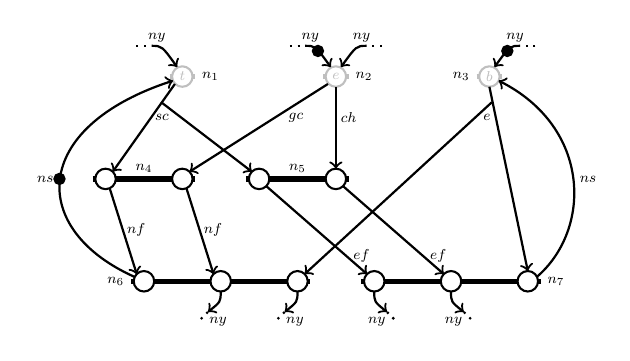
\begin{tikzpicture}[scale=0.65, every node/.style={transform shape}]

\begin{scope}[line width=2pt]
\draw (-1.75,-2) -- (0.25,-2);
\draw (1.25,-2) -- (3.25,-2);
\draw (-1,-4) -- (2.5,-4);
\draw (3.5,-4) -- (7,-4);
\end{scope}

\begin{scope}[line width=2pt, lightgray]
\draw (-0.25,0) -- (0.25,0);
\draw (2.75,0) -- (3.25,0);
\draw (5.75,0) -- (6.25,0);
\end{scope}

\filldraw [lightgray, fill=white]  (0,0)  circle (2mm) node (t0) {\footnotesize $t$};
\filldraw [lightgray, fill=white]  (3,0)  circle (2mm) node (e0) {\footnotesize $e$};
\filldraw [lightgray, fill=white]  (6,0)  circle (2mm) node (b0) {\footnotesize $b$};
\filldraw [fill=white]  (-1.5,-2)  circle (2mm) node (t1) {};
\filldraw [fill=white]  (0,-2)  circle (2mm) node (e1) {};
\filldraw [fill=white]  (1.5,-2)  circle (2mm) node (t2) {};
\filldraw [fill=white]  (3,-2)  circle (2mm) node (e2) {};
\filldraw [fill=white]  (-0.75,-4)  circle (2mm) node (t5) {};
\filldraw [fill=white]  (0.75,-4)  circle (2mm) node (e5) {};
\filldraw [fill=white]  (2.25,-4)  circle (2mm) node (b5) {};
\filldraw [fill=white]  (3.75,-4)  circle (2mm) node (t6) {};
\filldraw [fill=white]  (5.25,-4)  circle (2mm) node (e6) {};
\filldraw [fill=white]  (6.75,-4)  circle (2mm) node (b6) {};

\node at (0.55,0) {\footnotesize $n_1$};
\node at (3.55,0) {\footnotesize$n_2$};
\node at (5.45,0) {\footnotesize $n_3$};
\node at (-0.75,-1.8) {\footnotesize $n_4$};
\node at (2.25,-1.8) {\footnotesize $n_5$};
\node at (-1.3,-4) {\footnotesize $n_6$};
\node at (7.3,-4) {\footnotesize $n_7$};

\node at (-0.4, -0.8) {\footnotesize $sc$};
\node at (2.22, -0.8) {\footnotesize $gc$};
\node at (3.25, -0.8) {\footnotesize $ch$};
\node at (5.95, -0.8) {\footnotesize $e$};
\node at (-0.9,-3) {\footnotesize $nf$};
\node at (0.6, -3) {\footnotesize $nf$};
\node at (3.5,-3.5) {\footnotesize $ef$};
\node at (5,-3.5) {\footnotesize $ef$};
\node at (0.7, -4.8) {\footnotesize $ny$};
\node at (2.2, -4.8) {\footnotesize $ny$};
\node at (3.8, -4.8) {\footnotesize $ny$};
\node at (5.3, -4.8) {\footnotesize $ny$};
\node at (-0.5, 0.75) {\footnotesize $ny$};
\node at (2.5, 0.75) {\footnotesize $ny$};
\node at (3.5, 0.75) {\footnotesize $ny$};
\node at (6.5, 0.75) {\footnotesize $ny$};

\begin{scope}[thick,->]
\draw (-0.145, -0.145) -- (-1.36, -1.86); %t0-t1
\draw (-0.415, -0.5) -- (1.36, -1.86); %t0-t2
\draw (2.845, -0.145) -- (0.14, -1.86); %e0-e1
\draw (3, -0.2) -- (3, -1.8); %e0-e2
\draw (-1.5, -2) + (0.08, -0.18) -- (-0.89, -3.86); %t1-t3
\draw (0, -2) + (0.08, -0.18) -- (0.61, -3.86); %e1-e3
\draw (1.5, -2) + (0.145, -0.145) -- (3.61, -3.86); %t2-t4
\draw (3, -2) + (0.145, -0.145) -- (5.11, -3.86); %e2-e4
\draw (6.05, -0.5) -- (2.39, -3.86); %b0-b3
\draw (6, -0.2) -- (6.75, -3.8); %b0-b4
\draw (-0.92, -3.92) .. controls (-3, -3) and (-3, -1) .. (-0.18, -0.08) node [midway, left] {\footnotesize $ns$}; %t3-t0
\draw (6.92, -3.92) .. controls (8, -3) and (8, -1) .. (6.18, -0.08) node [midway, right] {\footnotesize $ns$}; %b4-b0
\draw (0.75,-4.2) .. controls (0.75, -4.4) .. (0.5,-4.6) ; %e3-e0
\draw (2.25, -4.2) .. controls (2.25, -4.4) .. (2, -4.6); %b3-b0
\draw (3.75, -4.2) .. controls (3.75, -4.4) .. (4, -4.6); %t4-t0
\draw (5.25, -4.2) .. controls (5.25, -4.4) .. (5.5, -4.6); %e4-e0
\draw (-0.6, 0.6) .. controls (-0.4, 0.6) .. (-0.1, 0.185); %t4-t0
\draw (2.4, 0.6) .. controls (2.6, 0.6) .. (2.9, 0.185); %e3-e0
\draw (3.6, 0.6) .. controls (3.4, 0.6) .. (3.1, 0.185); %e4-e0
\draw (6.6, 0.6) .. controls (6.4, 0.6) .. (6.1, 0.185); %b3-b0
\end{scope}

\begin{scope}[thick, dotted]
\draw (-0.9, 0.6) -- (-0.6, 0.6);
\draw (2.1, 0.6) -- (2.4, 0.6);
\draw (3.9, 0.6) -- (3.6, 0.6);
\draw (6.9, 0.6) -- (6.6, 0.6);
\draw (0.5,-4.6) -- (0.3, -4.8);
\draw (2, -4.6) -- (1.8, -4.8);
\draw (4, -4.6) -- (4.2, -4.8);
\draw (5.5, -4.6) -- (5.7, -4.8);
\end{scope}

\filldraw [fill=black]  (-2.4,-2)  circle (1mm);
\filldraw [fill=black]  (2.65,0.5)  circle (1mm);
\filldraw [fill=black]  (6.35,0.5)  circle (1mm);

\end{tikzpicture}
\end{minipage}
\begin{minipage}{.49\textwidth}
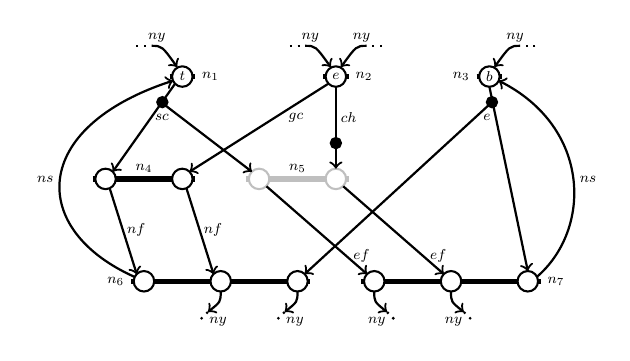
\begin{tikzpicture}[scale=0.65, every node/.style={transform shape}]

\begin{scope}[line width=2pt]
\draw (-0.25,0) -- (0.25,0);
\draw (2.75,0) -- (3.25,0);
\draw (5.75,0) -- (6.25,0);
\draw (-1.75,-2) -- (0.25,-2);
\draw (-1,-4) -- (2.5,-4);
\draw (3.5,-4) -- (7,-4);
\end{scope}

\draw [line width=2pt, lightgray] (1.25,-2) -- (3.25,-2);

\filldraw [fill=white]  (0,0)  circle (2mm) node (t0) {\footnotesize $t$};
\filldraw [fill=white]  (3,0)  circle (2mm) node (e0) {\footnotesize $e$};
\filldraw [fill=white]  (6,0)  circle (2mm) node (b0) {\footnotesize $b$};
\filldraw [fill=white]  (-1.5,-2)  circle (2mm) node (t1) {};
\filldraw [fill=white]  (0,-2)  circle (2mm) node (e1) {};
\filldraw [lightgray, fill=white]  (1.5,-2)  circle (2mm) node (t2) {};
\filldraw [lightgray, fill=white]  (3,-2)  circle (2mm) node (e2) {};
\filldraw [fill=white]  (-0.75,-4)  circle (2mm) node (t5) {};
\filldraw [fill=white]  (0.75,-4)  circle (2mm) node (e5) {};
\filldraw [fill=white]  (2.25,-4)  circle (2mm) node (b5) {};
\filldraw [fill=white]  (3.75,-4)  circle (2mm) node (t6) {};
\filldraw [fill=white]  (5.25,-4)  circle (2mm) node (e6) {};
\filldraw [fill=white]  (6.75,-4)  circle (2mm) node (b6) {};

\node at (0.55,0) {\footnotesize $n_1$};
\node at (3.55,0) {\footnotesize$n_2$};
\node at (5.45,0) {\footnotesize $n_3$};
\node at (-0.75,-1.8) {\footnotesize $n_4$};
\node at (2.25,-1.8) {\footnotesize $n_5$};
\node at (-1.3,-4) {\footnotesize $n_6$};
\node at (7.3,-4) {\footnotesize $n_7$};

\node at (-0.4, -0.8) {\footnotesize $sc$};
\node at (2.22, -0.8) {\footnotesize $gc$};
\node at (3.25, -0.8) {\footnotesize $ch$};
\node at (5.95, -0.8) {\footnotesize $e$};
\node at (-0.9,-3) {\footnotesize $nf$};
\node at (0.6, -3) {\footnotesize $nf$};
\node at (3.5,-3.5) {\footnotesize $ef$};
\node at (5,-3.5) {\footnotesize $ef$};
\node at (0.7, -4.8) {\footnotesize $ny$};
\node at (2.2, -4.8) {\footnotesize $ny$};
\node at (3.8, -4.8) {\footnotesize $ny$};
\node at (5.3, -4.8) {\footnotesize $ny$};
\node at (-0.5, 0.75) {\footnotesize $ny$};
\node at (2.5, 0.75) {\footnotesize $ny$};
\node at (3.5, 0.75) {\footnotesize $ny$};
\node at (6.5, 0.75) {\footnotesize $ny$};

\begin{scope}[thick,->]
\draw (-0.145, -0.145) -- (-1.36, -1.86); %t0-t1
\draw (-0.415, -0.5) -- (1.36, -1.86); %t0-t2
\draw (2.845, -0.145) -- (0.14, -1.86); %e0-e1
\draw (3, -0.2) -- (3, -1.8); %e0-e2
\draw (-1.5, -2) + (0.08, -0.18) -- (-0.89, -3.86); %t1-t3
\draw (0, -2) + (0.08, -0.18) -- (0.61, -3.86); %e1-e3
\draw (1.5, -2) + (0.145, -0.145) -- (3.61, -3.86); %t2-t4
\draw (3, -2) + (0.145, -0.145) -- (5.11, -3.86); %e2-e4
\draw (6.05, -0.5) -- (2.39, -3.86); %b0-b3
\draw (6, -0.2) -- (6.75, -3.8); %b0-b4
\draw (-0.92, -3.92) .. controls (-3, -3) and (-3, -1) .. (-0.18, -0.08) node [midway, left] {\footnotesize $ns$}; %t3-t0
\draw (6.92, -3.92) .. controls (8, -3) and (8, -1) .. (6.18, -0.08) node [midway, right] {\footnotesize $ns$}; %b4-b0
\draw (0.75,-4.2) .. controls (0.75, -4.4) .. (0.5,-4.6) ; %e3-e0
\draw (2.25, -4.2) .. controls (2.25, -4.4) .. (2, -4.6); %b3-b0
\draw (3.75, -4.2) .. controls (3.75, -4.4) .. (4, -4.6); %t4-t0
\draw (5.25, -4.2) .. controls (5.25, -4.4) .. (5.5, -4.6); %e4-e0
\draw (-0.6, 0.6) .. controls (-0.4, 0.6) .. (-0.1, 0.185); %t4-t0
\draw (2.4, 0.6) .. controls (2.6, 0.6) .. (2.9, 0.185); %e3-e0
\draw (3.6, 0.6) .. controls (3.4, 0.6) .. (3.1, 0.185); %e4-e0
\draw (6.6, 0.6) .. controls (6.4, 0.6) .. (6.1, 0.185); %b3-b0
\end{scope}

\begin{scope}[thick, dotted]
\draw (-0.9, 0.6) -- (-0.6, 0.6);
\draw (2.1, 0.6) -- (2.4, 0.6);
\draw (3.9, 0.6) -- (3.6, 0.6);
\draw (6.9, 0.6) -- (6.6, 0.6);
\draw (0.5,-4.6) -- (0.3, -4.8);
\draw (2, -4.6) -- (1.8, -4.8);
\draw (4, -4.6) -- (4.2, -4.8);
\draw (5.5, -4.6) -- (5.7, -4.8);
\end{scope}

\filldraw [fill=black]  (-0.39,-0.5)  circle (1mm);
\filldraw [fill=black]  (3,-1.3)  circle (1mm);
\filldraw [fill=black]  (6.05,-0.5)  circle (1mm);

\end{tikzpicture}
\end{minipage}
\begin{minipage}{.49\textwidth}
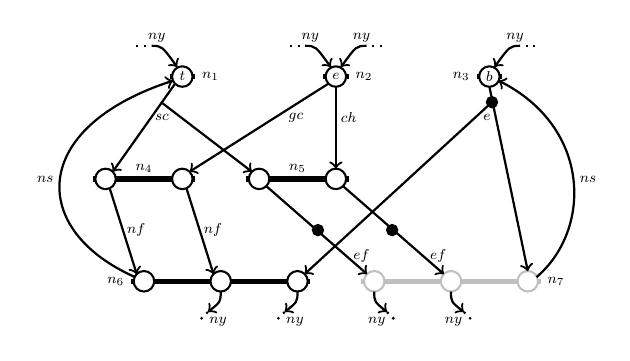
\begin{tikzpicture}[scale=0.65, every node/.style={transform shape}]

\begin{scope}[line width=2pt]
\draw (-0.25,0) -- (0.25,0);
\draw (2.75,0) -- (3.25,0);
\draw (5.75,0) -- (6.25,0);
\draw (-1.75,-2) -- (0.25,-2);
\draw (1.25,-2) -- (3.25,-2);
\draw (-1,-4) -- (2.5,-4);
\end{scope}

\draw [line width=2pt, lightgray] (3.5,-4) -- (7,-4);

\filldraw [fill=white]  (0,0)  circle (2mm) node (t0) {\footnotesize $t$};
\filldraw [fill=white]  (3,0)  circle (2mm) node (e0) {\footnotesize $e$};
\filldraw [fill=white]  (6,0)  circle (2mm) node (b0) {\footnotesize $b$};
\filldraw [fill=white]  (-1.5,-2)  circle (2mm) node (t1) {};
\filldraw [fill=white]  (0,-2)  circle (2mm) node (e1) {};
\filldraw [fill=white]  (1.5,-2)  circle (2mm) node (t2) {};
\filldraw [fill=white]  (3,-2)  circle (2mm) node (e2) {};
\filldraw [fill=white]  (-0.75,-4)  circle (2mm) node (t5) {};
\filldraw [fill=white]  (0.75,-4)  circle (2mm) node (e5) {};
\filldraw [fill=white]  (2.25,-4)  circle (2mm) node (b5) {};
\filldraw [lightgray, fill=white]  (3.75,-4)  circle (2mm) node (t6) {};
\filldraw [lightgray, fill=white]  (5.25,-4)  circle (2mm) node (e6) {};
\filldraw [lightgray, fill=white]  (6.75,-4)  circle (2mm) node (b6) {};

\node at (0.55,0) {\footnotesize $n_1$};
\node at (3.55,0) {\footnotesize$n_2$};
\node at (5.45,0) {\footnotesize $n_3$};
\node at (-0.75,-1.8) {\footnotesize $n_4$};
\node at (2.25,-1.8) {\footnotesize $n_5$};
\node at (-1.3,-4) {\footnotesize $n_6$};
\node at (7.3,-4) {\footnotesize $n_7$};

\node at (-0.4, -0.8) {\footnotesize $sc$};
\node at (2.22, -0.8) {\footnotesize $gc$};
\node at (3.25, -0.8) {\footnotesize $ch$};
\node at (5.95, -0.8) {\footnotesize $e$};
\node at (-0.9,-3) {\footnotesize $nf$};
\node at (0.6, -3) {\footnotesize $nf$};
\node at (3.5,-3.5) {\footnotesize $ef$};
\node at (5,-3.5) {\footnotesize $ef$};
\node at (0.7, -4.8) {\footnotesize $ny$};
\node at (2.2, -4.8) {\footnotesize $ny$};
\node at (3.8, -4.8) {\footnotesize $ny$};
\node at (5.3, -4.8) {\footnotesize $ny$};
\node at (-0.5, 0.75) {\footnotesize $ny$};
\node at (2.5, 0.75) {\footnotesize $ny$};
\node at (3.5, 0.75) {\footnotesize $ny$};
\node at (6.5, 0.75) {\footnotesize $ny$};

\begin{scope}[thick,->]
\draw (-0.145, -0.145) -- (-1.36, -1.86); %t0-t1
\draw (-0.415, -0.5) -- (1.36, -1.86); %t0-t2
\draw (2.845, -0.145) -- (0.14, -1.86); %e0-e1
\draw (3, -0.2) -- (3, -1.8); %e0-e2
\draw (-1.5, -2) + (0.08, -0.18) -- (-0.89, -3.86); %t1-t3
\draw (0, -2) + (0.08, -0.18) -- (0.61, -3.86); %e1-e3
\draw (1.5, -2) + (0.145, -0.145) -- (3.61, -3.86); %t2-t4
\draw (3, -2) + (0.145, -0.145) -- (5.11, -3.86); %e2-e4
\draw (6.05, -0.5) -- (2.39, -3.86); %b0-b3
\draw (6, -0.2) -- (6.75, -3.8); %b0-b4
\draw (-0.92, -3.92) .. controls (-3, -3) and (-3, -1) .. (-0.18, -0.08) node [midway, left] {\footnotesize $ns$}; %t3-t0
\draw (6.92, -3.92) .. controls (8, -3) and (8, -1) .. (6.18, -0.08) node [midway, right] {\footnotesize $ns$}; %b4-b0
\draw (0.75,-4.2) .. controls (0.75, -4.4) .. (0.5,-4.6) ; %e3-e0
\draw (2.25, -4.2) .. controls (2.25, -4.4) .. (2, -4.6); %b3-b0
\draw (3.75, -4.2) .. controls (3.75, -4.4) .. (4, -4.6); %t4-t0
\draw (5.25, -4.2) .. controls (5.25, -4.4) .. (5.5, -4.6); %e4-e0
\draw (-0.6, 0.6) .. controls (-0.4, 0.6) .. (-0.1, 0.185); %t4-t0
\draw (2.4, 0.6) .. controls (2.6, 0.6) .. (2.9, 0.185); %e3-e0
\draw (3.6, 0.6) .. controls (3.4, 0.6) .. (3.1, 0.185); %e4-e0
\draw (6.6, 0.6) .. controls (6.4, 0.6) .. (6.1, 0.185); %b3-b0
\end{scope}

\begin{scope}[thick, dotted]
\draw (-0.9, 0.6) -- (-0.6, 0.6);
\draw (2.1, 0.6) -- (2.4, 0.6);
\draw (3.9, 0.6) -- (3.6, 0.6);
\draw (6.9, 0.6) -- (6.6, 0.6);
\draw (0.5,-4.6) -- (0.3, -4.8);
\draw (2, -4.6) -- (1.8, -4.8);
\draw (4, -4.6) -- (4.2, -4.8);
\draw (5.5, -4.6) -- (5.7, -4.8);
\end{scope}

\filldraw [fill=black]  (2.65,-3)  circle (1mm);
\filldraw [fill=black]  (4.1,-3)  circle (1mm);
\filldraw [fill=black]  (6.05,-0.5)  circle (1mm);

\end{tikzpicture}
\end{minipage}
\begin{minipage}{.49\textwidth}
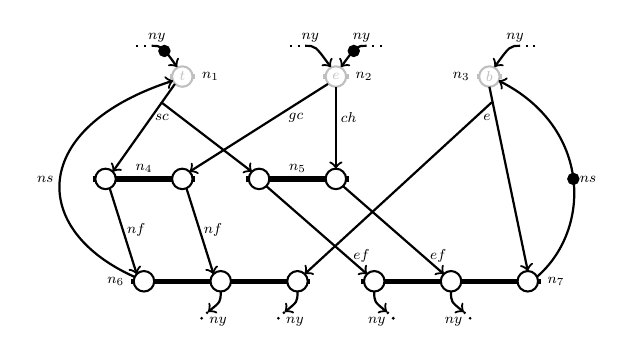
\begin{tikzpicture}[scale=0.65, every node/.style={transform shape}]

\begin{scope}[line width=2pt]
\draw (-1.75,-2) -- (0.25,-2);
\draw (1.25,-2) -- (3.25,-2);
\draw (-1,-4) -- (2.5,-4);
\draw (3.5,-4) -- (7,-4);
\end{scope}

\begin{scope}[line width=2pt, lightgray]
\draw (-0.25,0) -- (0.25,0);
\draw (2.75,0) -- (3.25,0);
\draw (5.75,0) -- (6.25,0);
\end{scope}

\filldraw [lightgray, fill=white]  (0,0)  circle (2mm) node (t0) {\footnotesize $t$};
\filldraw [lightgray, fill=white]  (3,0)  circle (2mm) node (e0) {\footnotesize $e$};
\filldraw [lightgray, fill=white]  (6,0)  circle (2mm) node (b0) {\footnotesize $b$};
\filldraw [fill=white]  (-1.5,-2)  circle (2mm) node (t1) {};
\filldraw [fill=white]  (0,-2)  circle (2mm) node (e1) {};
\filldraw [fill=white]  (1.5,-2)  circle (2mm) node (t2) {};
\filldraw [fill=white]  (3,-2)  circle (2mm) node (e2) {};
\filldraw [fill=white]  (-0.75,-4)  circle (2mm) node (t5) {};
\filldraw [fill=white]  (0.75,-4)  circle (2mm) node (e5) {};
\filldraw [fill=white]  (2.25,-4)  circle (2mm) node (b5) {};
\filldraw [fill=white]  (3.75,-4)  circle (2mm) node (t6) {};
\filldraw [fill=white]  (5.25,-4)  circle (2mm) node (e6) {};
\filldraw [fill=white]  (6.75,-4)  circle (2mm) node (b6) {};

\node at (0.55,0) {\footnotesize $n_1$};
\node at (3.55,0) {\footnotesize$n_2$};
\node at (5.45,0) {\footnotesize $n_3$};
\node at (-0.75,-1.8) {\footnotesize $n_4$};
\node at (2.25,-1.8) {\footnotesize $n_5$};
\node at (-1.3,-4) {\footnotesize $n_6$};
\node at (7.3,-4) {\footnotesize $n_7$};

\node at (-0.4, -0.8) {\footnotesize $sc$};
\node at (2.22, -0.8) {\footnotesize $gc$};
\node at (3.25, -0.8) {\footnotesize $ch$};
\node at (5.95, -0.8) {\footnotesize $e$};
\node at (-0.9,-3) {\footnotesize $nf$};
\node at (0.6, -3) {\footnotesize $nf$};
\node at (3.5,-3.5) {\footnotesize $ef$};
\node at (5,-3.5) {\footnotesize $ef$};
\node at (0.7, -4.8) {\footnotesize $ny$};
\node at (2.2, -4.8) {\footnotesize $ny$};
\node at (3.8, -4.8) {\footnotesize $ny$};
\node at (5.3, -4.8) {\footnotesize $ny$};
\node at (-0.5, 0.75) {\footnotesize $ny$};
\node at (2.5, 0.75) {\footnotesize $ny$};
\node at (3.5, 0.75) {\footnotesize $ny$};
\node at (6.5, 0.75) {\footnotesize $ny$};

\begin{scope}[thick,->]
\draw (-0.145, -0.145) -- (-1.36, -1.86); %t0-t1
\draw (-0.415, -0.5) -- (1.36, -1.86); %t0-t2
\draw (2.845, -0.145) -- (0.14, -1.86); %e0-e1
\draw (3, -0.2) -- (3, -1.8); %e0-e2
\draw (-1.5, -2) + (0.08, -0.18) -- (-0.89, -3.86); %t1-t3
\draw (0, -2) + (0.08, -0.18) -- (0.61, -3.86); %e1-e3
\draw (1.5, -2) + (0.145, -0.145) -- (3.61, -3.86); %t2-t4
\draw (3, -2) + (0.145, -0.145) -- (5.11, -3.86); %e2-e4
\draw (6.05, -0.5) -- (2.39, -3.86); %b0-b3
\draw (6, -0.2) -- (6.75, -3.8); %b0-b4
\draw (-0.92, -3.92) .. controls (-3, -3) and (-3, -1) .. (-0.18, -0.08) node [midway, left] {\footnotesize $ns$}; %t3-t0
\draw (6.92, -3.92) .. controls (8, -3) and (8, -1) .. (6.18, -0.08) node [midway, right] {\footnotesize $ns$}; %b4-b0
\draw (0.75,-4.2) .. controls (0.75, -4.4) .. (0.5,-4.6) ; %e3-e0
\draw (2.25, -4.2) .. controls (2.25, -4.4) .. (2, -4.6); %b3-b0
\draw (3.75, -4.2) .. controls (3.75, -4.4) .. (4, -4.6); %t4-t0
\draw (5.25, -4.2) .. controls (5.25, -4.4) .. (5.5, -4.6); %e4-e0
\draw (-0.6, 0.6) .. controls (-0.4, 0.6) .. (-0.1, 0.185); %t4-t0
\draw (2.4, 0.6) .. controls (2.6, 0.6) .. (2.9, 0.185); %e3-e0
\draw (3.6, 0.6) .. controls (3.4, 0.6) .. (3.1, 0.185); %e4-e0
\draw (6.6, 0.6) .. controls (6.4, 0.6) .. (6.1, 0.185); %b3-b0
\end{scope}

\begin{scope}[thick, dotted]
\draw (-0.9, 0.6) -- (-0.6, 0.6);
\draw (2.1, 0.6) -- (2.4, 0.6);
\draw (3.9, 0.6) -- (3.6, 0.6);
\draw (6.9, 0.6) -- (6.6, 0.6);
\draw (0.5,-4.6) -- (0.3, -4.8);
\draw (2, -4.6) -- (1.8, -4.8);
\draw (4, -4.6) -- (4.2, -4.8);
\draw (5.5, -4.6) -- (5.7, -4.8);
\end{scope}

\filldraw [fill=black]  (-0.35,0.5)  circle (1mm);
\filldraw [fill=black]  (3.35,0.5)  circle (1mm);
\filldraw [fill=black]  (7.64,-2)  circle (1mm);

\end{tikzpicture}
\end{minipage}
\begin{minipage}{.49\textwidth}
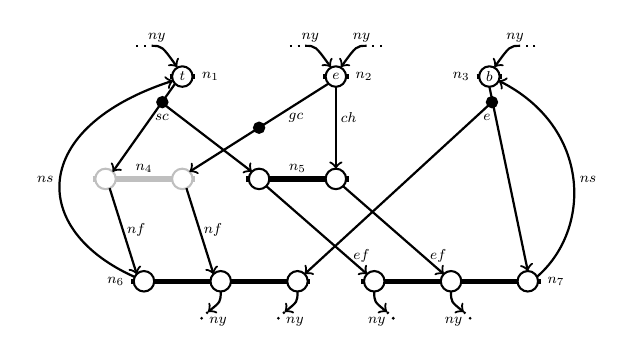
\begin{tikzpicture}[scale=0.65, every node/.style={transform shape}]

\begin{scope}[line width=2pt]
\draw (-0.25,0) -- (0.25,0);
\draw (2.75,0) -- (3.25,0);
\draw (5.75,0) -- (6.25,0);
\draw (1.25,-2) -- (3.25,-2);
\draw (-1,-4) -- (2.5,-4);
\draw (3.5,-4) -- (7,-4);
\end{scope}

\draw [line width=2pt, lightgray] (-1.75,-2) -- (0.25,-2);

\filldraw [fill=white]  (0,0)  circle (2mm) node (t0) {\footnotesize $t$};
\filldraw [fill=white]  (3,0)  circle (2mm) node (e0) {\footnotesize $e$};
\filldraw [fill=white]  (6,0)  circle (2mm) node (b0) {\footnotesize $b$};
\filldraw [lightgray, fill=white]  (-1.5,-2)  circle (2mm) node (t1) {};
\filldraw [lightgray, fill=white]  (0,-2)  circle (2mm) node (e1) {};
\filldraw [fill=white]  (1.5,-2)  circle (2mm) node (t2) {};
\filldraw [fill=white]  (3,-2)  circle (2mm) node (e2) {};
\filldraw [fill=white]  (-0.75,-4)  circle (2mm) node (t5) {};
\filldraw [fill=white]  (0.75,-4)  circle (2mm) node (e5) {};
\filldraw [fill=white]  (2.25,-4)  circle (2mm) node (b5) {};
\filldraw [fill=white]  (3.75,-4)  circle (2mm) node (t6) {};
\filldraw [fill=white]  (5.25,-4)  circle (2mm) node (e6) {};
\filldraw [fill=white]  (6.75,-4)  circle (2mm) node (b6) {};

\node at (0.55,0) {\footnotesize $n_1$};
\node at (3.55,0) {\footnotesize$n_2$};
\node at (5.45,0) {\footnotesize $n_3$};
\node at (-0.75,-1.8) {\footnotesize $n_4$};
\node at (2.25,-1.8) {\footnotesize $n_5$};
\node at (-1.3,-4) {\footnotesize $n_6$};
\node at (7.3,-4) {\footnotesize $n_7$};

\node at (-0.4, -0.8) {\footnotesize $sc$};
\node at (2.22, -0.8) {\footnotesize $gc$};
\node at (3.25, -0.8) {\footnotesize $ch$};
\node at (5.95, -0.8) {\footnotesize $e$};
\node at (-0.9,-3) {\footnotesize $nf$};
\node at (0.6, -3) {\footnotesize $nf$};
\node at (3.5,-3.5) {\footnotesize $ef$};
\node at (5,-3.5) {\footnotesize $ef$};
\node at (0.7, -4.8) {\footnotesize $ny$};
\node at (2.2, -4.8) {\footnotesize $ny$};
\node at (3.8, -4.8) {\footnotesize $ny$};
\node at (5.3, -4.8) {\footnotesize $ny$};
\node at (-0.5, 0.75) {\footnotesize $ny$};
\node at (2.5, 0.75) {\footnotesize $ny$};
\node at (3.5, 0.75) {\footnotesize $ny$};
\node at (6.5, 0.75) {\footnotesize $ny$};

\begin{scope}[thick,->]
\draw (-0.145, -0.145) -- (-1.36, -1.86); %t0-t1
\draw (-0.415, -0.5) -- (1.36, -1.86); %t0-t2
\draw (2.845, -0.145) -- (0.14, -1.86); %e0-e1
\draw (3, -0.2) -- (3, -1.8); %e0-e2
\draw (-1.5, -2) + (0.08, -0.18) -- (-0.89, -3.86); %t1-t3
\draw (0, -2) + (0.08, -0.18) -- (0.61, -3.86); %e1-e3
\draw (1.5, -2) + (0.145, -0.145) -- (3.61, -3.86); %t2-t4
\draw (3, -2) + (0.145, -0.145) -- (5.11, -3.86); %e2-e4
\draw (6.05, -0.5) -- (2.39, -3.86); %b0-b3
\draw (6, -0.2) -- (6.75, -3.8); %b0-b4
\draw (-0.92, -3.92) .. controls (-3, -3) and (-3, -1) .. (-0.18, -0.08) node [midway, left] {\footnotesize $ns$}; %t3-t0
\draw (6.92, -3.92) .. controls (8, -3) and (8, -1) .. (6.18, -0.08) node [midway, right] {\footnotesize $ns$}; %b4-b0
\draw (0.75,-4.2) .. controls (0.75, -4.4) .. (0.5,-4.6) ; %e3-e0
\draw (2.25, -4.2) .. controls (2.25, -4.4) .. (2, -4.6); %b3-b0
\draw (3.75, -4.2) .. controls (3.75, -4.4) .. (4, -4.6); %t4-t0
\draw (5.25, -4.2) .. controls (5.25, -4.4) .. (5.5, -4.6); %e4-e0
\draw (-0.6, 0.6) .. controls (-0.4, 0.6) .. (-0.1, 0.185); %t4-t0
\draw (2.4, 0.6) .. controls (2.6, 0.6) .. (2.9, 0.185); %e3-e0
\draw (3.6, 0.6) .. controls (3.4, 0.6) .. (3.1, 0.185); %e4-e0
\draw (6.6, 0.6) .. controls (6.4, 0.6) .. (6.1, 0.185); %b3-b0
\end{scope}

\begin{scope}[thick, dotted]
\draw (-0.9, 0.6) -- (-0.6, 0.6);
\draw (2.1, 0.6) -- (2.4, 0.6);
\draw (3.9, 0.6) -- (3.6, 0.6);
\draw (6.9, 0.6) -- (6.6, 0.6);
\draw (0.5,-4.6) -- (0.3, -4.8);
\draw (2, -4.6) -- (1.8, -4.8);
\draw (4, -4.6) -- (4.2, -4.8);
\draw (5.5, -4.6) -- (5.7, -4.8);
\end{scope}

\filldraw [fill=black]  (-0.39,-0.5)  circle (1mm);
\filldraw [fill=black]  (1.5,-1)  circle (1mm);
\filldraw [fill=black]  (6.05,-0.5)  circle (1mm);

\end{tikzpicture}
\end{minipage}
\begin{minipage}{.49\textwidth}
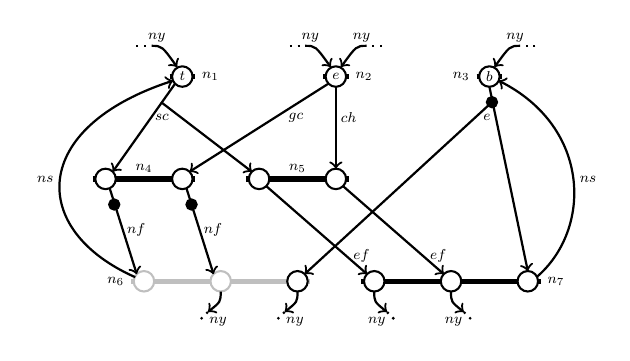
\begin{tikzpicture}[scale=0.65, every node/.style={transform shape}]

\begin{scope}[line width=2pt]
\draw (-0.25,0) -- (0.25,0);
\draw (2.75,0) -- (3.25,0);
\draw (5.75,0) -- (6.25,0);
\draw (-1.75,-2) -- (0.25,-2);
\draw (1.25,-2) -- (3.25,-2);
\draw (3.5,-4) -- (7,-4);
\end{scope}

\draw [line width=2pt, lightgray] (-1,-4) -- (2.5,-4);

\filldraw [fill=white]  (0,0)  circle (2mm) node (t0) {\footnotesize $t$};
\filldraw [fill=white]  (3,0)  circle (2mm) node (e0) {\footnotesize $e$};
\filldraw [fill=white]  (6,0)  circle (2mm) node (b0) {\footnotesize $b$};
\filldraw [fill=white]  (-1.5,-2)  circle (2mm) node (t1) {};
\filldraw [fill=white]  (0,-2)  circle (2mm) node (e1) {};
\filldraw [fill=white]  (1.5,-2)  circle (2mm) node (t2) {};
\filldraw [fill=white]  (3,-2)  circle (2mm) node (e2) {};
\filldraw [lightgray, fill=white]  (-0.75,-4)  circle (2mm) node (t5) {};
\filldraw [lightgray, fill=white]  (0.75,-4)  circle (2mm) node (e5) {};
\filldraw [fill=white]  (2.25,-4)  circle (2mm) node (b5) {};
\filldraw [fill=white]  (3.75,-4)  circle (2mm) node (t6) {};
\filldraw [fill=white]  (5.25,-4)  circle (2mm) node (e6) {};
\filldraw [fill=white]  (6.75,-4)  circle (2mm) node (b6) {};

\node at (0.55,0) {\footnotesize $n_1$};
\node at (3.55,0) {\footnotesize$n_2$};
\node at (5.45,0) {\footnotesize $n_3$};
\node at (-0.75,-1.8) {\footnotesize $n_4$};
\node at (2.25,-1.8) {\footnotesize $n_5$};
\node at (-1.3,-4) {\footnotesize $n_6$};
\node at (7.3,-4) {\footnotesize $n_7$};

\node at (-0.4, -0.8) {\footnotesize $sc$};
\node at (2.22, -0.8) {\footnotesize $gc$};
\node at (3.25, -0.8) {\footnotesize $ch$};
\node at (5.95, -0.8) {\footnotesize $e$};
\node at (-0.9,-3) {\footnotesize $nf$};
\node at (0.6, -3) {\footnotesize $nf$};
\node at (3.5,-3.5) {\footnotesize $ef$};
\node at (5,-3.5) {\footnotesize $ef$};
\node at (0.7, -4.8) {\footnotesize $ny$};
\node at (2.2, -4.8) {\footnotesize $ny$};
\node at (3.8, -4.8) {\footnotesize $ny$};
\node at (5.3, -4.8) {\footnotesize $ny$};
\node at (-0.5, 0.75) {\footnotesize $ny$};
\node at (2.5, 0.75) {\footnotesize $ny$};
\node at (3.5, 0.75) {\footnotesize $ny$};
\node at (6.5, 0.75) {\footnotesize $ny$};

\begin{scope}[thick,->]
\draw (-0.145, -0.145) -- (-1.36, -1.86); %t0-t1
\draw (-0.415, -0.5) -- (1.36, -1.86); %t0-t2
\draw (2.845, -0.145) -- (0.14, -1.86); %e0-e1
\draw (3, -0.2) -- (3, -1.8); %e0-e2
\draw (-1.5, -2) + (0.08, -0.18) -- (-0.89, -3.86); %t1-t3
\draw (0, -2) + (0.08, -0.18) -- (0.61, -3.86); %e1-e3
\draw (1.5, -2) + (0.145, -0.145) -- (3.61, -3.86); %t2-t4
\draw (3, -2) + (0.145, -0.145) -- (5.11, -3.86); %e2-e4
\draw (6.05, -0.5) -- (2.39, -3.86); %b0-b3
\draw (6, -0.2) -- (6.75, -3.8); %b0-b4
\draw (-0.92, -3.92) .. controls (-3, -3) and (-3, -1) .. (-0.18, -0.08) node [midway, left] {\footnotesize $ns$}; %t3-t0
\draw (6.92, -3.92) .. controls (8, -3) and (8, -1) .. (6.18, -0.08) node [midway, right] {\footnotesize $ns$}; %b4-b0
\draw (0.75,-4.2) .. controls (0.75, -4.4) .. (0.5,-4.6) ; %e3-e0
\draw (2.25, -4.2) .. controls (2.25, -4.4) .. (2, -4.6); %b3-b0
\draw (3.75, -4.2) .. controls (3.75, -4.4) .. (4, -4.6); %t4-t0
\draw (5.25, -4.2) .. controls (5.25, -4.4) .. (5.5, -4.6); %e4-e0
\draw (-0.6, 0.6) .. controls (-0.4, 0.6) .. (-0.1, 0.185); %t4-t0
\draw (2.4, 0.6) .. controls (2.6, 0.6) .. (2.9, 0.185); %e3-e0
\draw (3.6, 0.6) .. controls (3.4, 0.6) .. (3.1, 0.185); %e4-e0
\draw (6.6, 0.6) .. controls (6.4, 0.6) .. (6.1, 0.185); %b3-b0
\end{scope}

\begin{scope}[thick, dotted]
\draw (-0.9, 0.6) -- (-0.6, 0.6);
\draw (2.1, 0.6) -- (2.4, 0.6);
\draw (3.9, 0.6) -- (3.6, 0.6);
\draw (6.9, 0.6) -- (6.6, 0.6);
\draw (0.5,-4.6) -- (0.3, -4.8);
\draw (2, -4.6) -- (1.8, -4.8);
\draw (4, -4.6) -- (4.2, -4.8);
\draw (5.5, -4.6) -- (5.7, -4.8);
\end{scope}

\filldraw [fill=black]  (-1.33,-2.5)  circle (1mm);
\filldraw [fill=black]  (0.18,-2.5)  circle (1mm);
\filldraw [fill=black]  (6.05,-0.5)  circle (1mm);

\end{tikzpicture}
\end{minipage}
\caption{A possible run of the negotiation in Figure~\ref{fig:pollination}. Tokens represent the current readiness of each process. Gray nodes denote enabled nodes. The run illustrates how choices at \(n_1\), \(n_2\), and \(n_3\) propagate to subsequent flowering and synchronization behaviour.}
\label{fig:run}
\end{figure}

\smallskip
As in other state-based models, one can define the \emph{reachability graph} of a negotiation: its vertices are all markings reachable from the initial marking \(x_0\), and there is an edge from \(x\) to \(x'\) labelled \((n,r)\) whenever \(x \xrightarrow{(n,r)} x'\). Figure~\ref{fig:rg-pol} depicts part of the reachability graph corresponding to the negotiation fragment in Figure~\ref{fig:pollination}.

\begin{figure}[t]
\centering
\begin{tikzpicture}[scale=0.6, every node/.style={transform shape}]

\node at (0,0) {$\{\{n_1\}, \{n_2\}, \{n_3\}\}$};
\node at (-6,-3) {$\{\{n_4, n_5\}, \{n_2\}, \{n_3\}\}$};
\node at (-2,-3) {$\{\{n_1\}, \{n_4\}, \{n_3\}\}$};
\node at (2,-3) {$\{\{n_1\}, \{n_5\}, \{n_3\}\}$};
\node at (6,-3) {$\{\{n_1\}, \{n_2\}, \{n_6, n_7\}\}$};
\node at (-10,-6) {$\{\{n_4, n_5\}, \{n_4\}, \{n_3\}\}$};
\node at (-5,-6) {$\{\{n_4, n_5\}, \{n_5\}, \{n_3\}\}$};
\node at (0,-6) {$\{\{n_4, n_5\}, \{n_2\}, \{n_6, n_7\}\}$};
\node at (5,-6) {$\{\{n_1\}, \{n_4\}, \{n_6, n_7\}\}$};
\node at (10,-6) {$\{\{n_1\}, \{n_5\}, \{n_6, n_7\}\}$};
\node at (-9,-9) {$\{\{n_6\}, \{n_6\}, \{n_3\}\}$};
\node at (3,-9) {$\{\{n_4, n_5\}, \{n_4\}, \{n_6, n_7\}\}$};
\node at (-3,-9) {$\{\{n_7\}, \{n_7\}, \{n_3\}\}$};
\node at (9,-9) {$\{\{n_4, n_5\}, \{n_5\}, \{n_6, n_7\}\}$};
\node at (-6,-12) {$\{\{n_6\}, \{n_6\}, \{n_6, n_7\}\}$};
\node at (6,-12) {$\{\{n_7\}, \{n_7\}, \{n_6, n_7\}\}$};

\begin{scope}[-Stealth]
\draw (0,-0.3) -- (-6,-2.7) node [midway, left, above] {\footnotesize $(n_1, sc)$};
\draw (0,-0.3) -- (-2,-2.7) node [midway, left] {\footnotesize $(n_2, gc)$};
\draw (0,-0.3) -- (2,-2.7) node [midway, left] {\footnotesize $(n_2, ch)$};
\draw (0,-0.3) -- (6,-2.7) node [midway, right, above] {\footnotesize $(n_3, e)$};
\draw (-6,-3.3) -- (-10,-5.7) node [midway, left] {\footnotesize $(n_2, gc)$};
\draw (-6,-3.3) -- (-5,-5.7) node [midway, left, above] {\footnotesize $(n_2, ch)$};%
\draw (-6,-3.3) -- (-0.25,-5.7) node [midway, left] {\footnotesize $(n_3, e)$};
\draw (-2,-3.3) -- (-9.5,-5.7) node [midway, left, below] {\footnotesize $(n_1, sc)$};%
\draw (-2,-3.3) -- (4.75,-5.7) node [midway, left] {\footnotesize $(n_3, e)$};
\draw (2,-3.3) -- (-4.5,-5.7) node [midway, left, below] {\footnotesize $(n_1, sc)$};%
\draw (2,-3.3) -- (9.5,-5.7) node [midway, left] {\footnotesize $(n_3, e)$};
\draw (6,-3.3) -- (0.25,-5.7) node [midway, left] {\footnotesize $(n_1, sc)$};
\draw (6,-3.3) -- (5.25,-5.7) node [midway, left, above] {\footnotesize $(n_2, gc)$};%
\draw (6,-3.3) -- (10,-5.7) node [midway, left] {\footnotesize $(n_2, ch)$};
\draw (-10,-6.3) -- (-9,-8.7) node [midway, left] {\footnotesize $(n_4, nf)$};
\draw (-10,-6.3) -- (2.5,-8.7) node [midway, left] {\footnotesize $(n_3, e)$};
\draw (-5,-6.3) -- (-3,-8.7) node [midway, left] {\footnotesize $(n_4, nf)$};
\draw (-5,-6.3) -- (8.5,-8.7) node [midway, left] {\footnotesize $(n_3, e)$};
\draw (0,-6.3) -- (2.75,-8.7) node [midway, left] {\footnotesize $(n_4, nf)$};
\draw (0,-6.3) -- (8.75,-8.7) node [midway, left] {\footnotesize $(n_3, e)$};
\draw (5,-6.3) -- (3,-8.7) node [midway, left] {\footnotesize $(n_4, nf)$};
\draw (10,-6.3) -- (9,-8.7) node [midway, left] {\footnotesize $(n_4, nf)$};
\draw (-9,-9.3) -- (-6,-11.7) node [midway, left] {\footnotesize $(n_4, nf)$};
\draw (-3,-9.3) -- (5.5,-11.7) node [midway, left] {\footnotesize $(n_4, nf)$};
\draw (3,-9.3) -- (-5.5,-11.7) node [midway, left] {\footnotesize $(n_4, nf)$};
\draw (9,-9.3) -- (6,-11.7) node [midway, left] {\footnotesize $(n_4, nf)$};
\draw (-8, -12) .. controls (-15, -9) and (-15, -1) .. (-2, 0);
\draw (8, -12) .. controls (15, -9) and (15, -1) .. (2, 0);
\end{scope}

\end{tikzpicture}
\caption{Part of the reachability graph for the negotiation in Figure~\ref{fig:pollination}. Each vertex is a marking (represented symbolically), and edges are labelled by occurring outcomes \((n,r)\). The number of reachable markings can grow exponentially in the number of nodes due to hyperarc branching.}
\label{fig:rg-pol}
\end{figure}

In general, occurrence sequences can be arbitrarily long, and the number of reachable markings can be very large. For negotiations with multiple hyperarcs, each with branching degree \(n\), the number of distinct branching patterns can grow as \(n^k\), where \(k\) is the number of hyperarcs, leading to an exponential blow-up in the marking graph. It is known that the reachability problem for negotiations is PSPACE-complete in general, and already coNP-hard and in DP for acyclic negotiations (see, e.g.,~\cite{EsparzaDeselNegotiations}).

\paragraph{Key observations from this example.}
This example illustrates several features of negotiations:
\begin{enumerate}
\item \textbf{Multiparty interactions are atomic:} An interaction involves all its participating agents simultaneously and cannot be decomposed into pairwise steps. Node \(n_6\) requires all three processes to participate simultaneously.
\item \textbf{Synchronization is explicit, not emergent:} Agents synchronize because the model says so, not because of shared state.
\item \textbf{Independence is visible in the structure:} Disjoint sets of agents can proceed independently, and this is evident in the graph itself. Nodes \(n_1\), \(n_2\) and \(n_3\) can occur in either order, or even conceptually ``at the same time'' since they involve disjoint sets of processes.
\item \textbf{Non-determinism:} After \(n_1\), \(t\) is ready to engage in both \(n_4\) and \(n_5\) and the choice is resolved only through interaction.
\item \textbf{Control flow is global, not agent-local:} Choices made at one node propagate to future possibilities for all involved agents.
\item \textbf{Information transfer:} The example highlights that synchronization itself acts as a mechanism for
information flow between agents -- by participating in a joint interaction, agents
implicitly exchange information that influences future behavior, even though no
explicit shared state or data is modeled.
\item \textbf{Succicntness:} The underlying reachability graph could be exponential on the number of nodes.
\end{enumerate}

Negotiations have been applied to the analysis of business processes, often modelled by workflow Petri nets~\cite{EsparzaWorkflow}. Such nets underlie popular graphical notations like BPMN, EPC, and UML Activity Diagrams~\cite{DijkmanBPMN}. Deterministic negotiations are closely related to free-choice workflow nets~\cite{EsparzaFreeChoice}, which are expressive enough for many industrial processes; empirical studies show that a large fraction of real-world models fall into the free-choice class.

In the remainder of the thesis, we extend negotiations with quantitative timing information, in the form of local clocks and time constraints, and study reachability in this enriched model.

%_____________________________________________________________________________

\section{Local-Timed Negotiations}

This thesis studies \emph{local-timed negotiations} (LTNs)~\cite{LTNOriginal}, which combine the multiparty synchronization structure of negotiations with quantitative timing constraints inspired by timed automata.

\subsection{Key Ideas}

Each agent in an LTN maintains its own \emph{local reference time}, evolving independently. Like timed automata, each agent has a set of \emph{local clocks} measuring elapsed time. Outcomes can be annotated with:
\begin{itemize}
\item \textbf{Guards}: Constraints on local clocks (e.g., $x \geq 5$, $y < 10$)
\item \textbf{Resets}: Clocks to reset to zero when the outcome occurs
\end{itemize}

The crucial new feature is \emph{explicit time synchronization}. Some interactions may \emph{synchronize} the local reference times of participating agents, aligning their clocks. Other interactions leave local times independent. This creates a spectrum between fully asynchronous systems (no synchronization) and tightly coupled systems (frequent synchronization).

\paragraph{Why Local Time?} The local-time approach offers several advantages:
\begin{enumerate}
\item \textbf{Explicit independence}: When two nodes involve disjoint agent sets and neither synchronizes time, they are genuinely independent and can be reordered freely.
\item \textbf{Realistic modeling}: In distributed systems, components often have their own clocks (e.g., different computers, different sensors). Local time reflects this reality.
\item \textbf{Partial-order potential}: Explicit independence enables partial-order reduction techniques, potentially avoiding exploration of redundant interleavings.
\item \textbf{Flexible synchronization}: The model supports both tightly synchronized systems (e.g., real-time embedded systems with global clock) and loosely coupled systems (e.g., distributed protocols with occasional synchronization).
\end{enumerate}

\paragraph{Why not assume global time?}
A natural question is why we do not assume a single global time shared by all
agents, as is standard in timed automata and their networks. Under such a
global-time semantics, timed negotiations collapse to a classical timed automaton
obtained as the synchronous product of the agents’ local timed behaviors: all
clocks advance uniformly, interactions implicitly synchronize time, and
reachability reduces to standard timed-automata reachability analyzable via region
or zone-based techniques.

This global-time assumption fundamentally alters the concurrency model. Independent
agents can no longer progress at different rates, and relative delays between
agents do not persist across interactions. As a result, the semantics collapses
from an interaction-centric concurrent model to an interleaving-based model with
global temporal coordination.

Local-timed negotiations deliberately reject this assumption. By allowing agents
to maintain independent reference times, the model preserves structural
independence and makes temporal coordination explicit. This semantic freedom is
essential for the expressiveness of the model and for isolating the boundary
between decidability and undecidability explored in this thesis.

\subsection{The Challenge of Mixed Synchronization}

Allowing arbitrary mixtures of time-synchronizing and non-synchronizing interactions creates a powerful but complex model. The interplay between independent local clocks and selective synchronization can simulate sophisticated computational behaviors. As we will show, this generality comes at a cost: reachability becomes undecidable.

However, by imposing restrictions on synchronization patterns, clock usage, or behavioral properties, we can recover decidability. Understanding which restrictions suffice—and which do not—is the central technical challenge of this thesis.
%_____________________________________________________________________________

\section{Contributions}

This thesis provides the first systematic study of decidability and complexity for reachability in local-timed negotiations. Our main contributions are:

\subsection{Undecidability of General LTNs}

We prove that reachability is \emph{undecidable} for LTNs that permit arbitrary mixtures of time-synchronizing and non-synchronizing interactions. The proof uses a reduction from the halting problem for two-counter machines, showing that LTNs with mixed synchronization can encode unbounded computation. This establishes a sharp boundary: full generality leads to undecidability.

\subsection{Two PSPACE-Complete Structural Fragments}

We identify two extreme fragments where reachability is decidable and PSPACE-complete:

\paragraph{Synchronization-free LTNs.} When \emph{no} interactions synchronize local times, agents evolve completely independently. We show that reachability remains PSPACE-complete. The proof constructs a suitable region abstraction that accounts for local timing constraints without global coordination.

\paragraph{Fully-synchronizing LTNs.} When \emph{all} interactions synchronize local times, the system behaves like a classical timed automaton with global time. We again obtain PSPACE-completeness, connecting to known complexity results for timed automata.

These results delineate the extremes of the synchronization spectrum and provide baseline complexity bounds.

\subsection{Decidability via Drift-Boundedness}

We introduce a semantic restriction called \emph{drift-boundedness}. An LTN is drift-bounded by constant $K$ if in every behavior, the difference between local times of any two agents (the \emph{drift}) never exceeds $K$. Intuitively, even though agents have independent clocks, their times cannot diverge too far.

We prove that reachability is \emph{decidable} for drift-bounded LTNs. The key insight is to construct a region automaton over the untimed marking graph, where regions bound not only clock values but also inter-agent time differences. Drift-boundedness ensures this abstraction is finite and sound.

Drift-boundedness is inspired by similar notions for networks of timed automata~\cite{DriftTA1,DriftTA2}. Our contribution is adapting this concept to the negotiation setting and proving decidability.

\subsection{Decidability via Connected Communication}

We define a syntactic fragment called \emph{connectedly-communicating LTNs}. Informally, an LTN is connectedly-communicating if in every cycle of the marking graph, each agent synchronizes (directly or indirectly) with every other agent through time-synchronizing interactions.

We formalize this using \emph{communication graphs} associated with loops in the marking graph. A loop is connectedly-communicating if its communication graph is connected. We prove that if \emph{all} loops are connectedly-communicating, then reachability is decidable.

The intuition is that frequent synchronization prevents unbounded drift and limits the computational power of the system. This fragment is inspired by restrictions in hierarchical message sequence charts~\cite{HenriksenMSG} and distributed controller synthesis~\cite{PnueliRosner}, adapted to our negotiation-based setting.

\subsection{Summary of Landscape}

Our results provide a comprehensive picture of decidability for LTN reachability:

\begin{center}
\begin{tabular}{lcc}
\toprule
\textbf{Fragment} & \textbf{Reachability} \\
\midrule
General LTNs (mixed synchronization) & Undecidable \\
Synchronization-free LTNs & Decidable \\
Fully-synchronizing LTNs & Decidable \\
Drift-bounded LTNs & Decidable \\
Connectedly-communicating LTNs & Decidable \\
\bottomrule
\end{tabular}
\end{center}

%_____________________________________________________________________________

\section{Organization of the thesis}
\label{sec:organization}

The thesis is structured in two main parts.

\medskip
\noindent\textbf{Part~I: Modelling local-timed negotiations and undecidability.}

\begin{itemize}
  \item \textbf{Chapter~\ref{chap:preliminaries}} introduces the basic notions and notations used throughout the thesis. We recall the definitions of negotiations, timed automata, and networks of timed automata, accompanied by illustrative examples.
  \item \textbf{Chapter~\ref{chap:ltn}} defines local-timed negotiations formally. We develop their semantics, introduce local clocks and time-synchronizing interactions, and show that reachability is undecidable in the general LTN model.
\end{itemize}

\medskip
\noindent\textbf{Part~II: Decidable subclasses of local-timed negotiations.}

\begin{itemize}
  \item \textbf{Chapter~\ref{chap:synch-fragments}} studies two extreme structural fragments of LTNs: synchronization-free negotiations and always-synchronizing negotiations. We prove that reachability is PSPACE-complete in both cases.
  \item \textbf{Chapter~\ref{chap:drift-bounded}} introduces drift-bounded LTNs. We formalize drift-boundedness, study its algorithmic properties, and show that reachability is decidable in this fragment via a region-based construction over untimed behaviours.
  \item \textbf{Chapter~\ref{chap:connected-communicating}} presents the fragment of connectedly-communicating LTNs. We formalize the associated communication graphs, prove decidability of reachability, and discuss potential extensions to weaker communication assumptions.
\end{itemize}

\medskip
Each chapter concludes with a section of \emph{concluding remarks}, summarizing the main definitions and results and providing pointers to later chapters where they are used.

\paragraph{Conceptual takeaway.}
The results developed in this thesis can be understood as exploring a design space
organized along three independent axes. 

\begin{enumerate}
\item The first axis is \emph{temporal coupling}: whether agents evolve with respect to a single global time or maintain independent local reference times. 
\item The second axis is \emph{synchronization strength}, ranging from no synchronization, through selective synchronization at chosen interactions, to mandatory synchronization at every interaction. 
\item The third axis is the \emph{persistence of timing information}: whether relative timing differences between agents can accumulate and persist across interactions or are periodically eliminated by synchronization.
\end{enumerate}
Local-timed negotiations inhabit the region of this space where
time is local, synchronization is explicit and optional, and relative timing
information can persist. The remainder of the thesis shows how different restrictions
along these axes delineate the precise boundary between decidability and
undecidability of reachability.
%_____________________________________________________________________________

\section{Related work}
\label{sec:related}

We briefly survey work related to local-time semantics, timed models of concurrency, negotiation models, and decidable fragments in distributed systems.

\paragraph{Local-time semantics and timed automata.}
A local-time semantics was proposed for networks of timed automata in~\cite{LocalTimeTA}. Recently, this semantics has been used for zone-based verification of reachability properties~\cite{LocalZone1,LocalZone2} and B\"uchi reachability~\cite{LocalBuchi}. Local-time semantics has also been investigated as a foundation for applying partial-order methods to timed automata. In networks of timed automata, independence between actions becomes more explicit under local-time semantics, leading to zone graphs that contain ``diamonds'' corresponding to commuting actions, which can mitigate the combinatorial explosion due to interleavings.

In contrast, our work starts from local-time semantics as a primitive feature, and makes synchronization an explicit option at the level of the negotiation model. This emphasises independence and true concurrency in the presence of time.

\paragraph{Timed models mixing concurrency and timing.}
A variety of models extend classical concurrency formalisms with timing information, including time Petri nets~\cite{MerlinTimePN}, timed-arc Petri nets~\cite{HansenTimedArc}, and time-constrained message sequence charts~\cite{AlurMSC}. Each provides a different balance between expressiveness and tractability. Partial-order semantics for such models have also been explored, for example via unfoldings and finite complete prefixes~\cite{EsparzaUnfoldings,KhomenkoTimePN}.

To the best of our knowledge, real-time extensions of negotiations have not been systematically studied before the introduction of local-timed negotiations in~\cite{LTNOriginal}.

\paragraph{Negotiations and concurrency theory.}
Negotiations were introduced in~\cite{EsparzaDeselNegotiations} as a primitive model of concurrency rooted in atomic multiparty interactions. They have been related to workflow Petri nets and business process models~\cite{EsparzaWorkflow,EsparzaFreeChoice}, and studied in terms of soundness, summarization, and complexity. The notion of atomic negotiations and occurrence sequences provides a natural setting for partial-order reasoning.

\paragraph{Bounded drift and partial-order methods.}
The idea of bounding the drift between local times of processes has been studied for networks of timed automata in~\cite{DriftTA1,DriftTA2}. In that setting, drift-boundedness is used to design simulation techniques and to ensure the finiteness of certain abstractions in zone-based verification. Our drift-boundedness notion for LTNs is analogous in spirit, but tailored to the negotiation model and its marking-based semantics.

Partial-order semantics for timed systems, including time Petri nets and timed automata, have been investigated in~\cite{EsparzaUnfoldings,KhomenkoTimePN,LocalBuchi}. These works show that combining timing with partial orders can retain enough structure for efficient verification. Our work aims at a similar goal in the context of negotiations.

\paragraph{Connected communication and decidable fragments.}
The connectedly-communicating fragment of LTNs is inspired by the The MSO theory of connectedly communicating processes~\cite{}. Similar restrictions has been studied in hierarchical message sequence charts~\cite{HenriksenMSG}, where communication structure enforces decidability of the emptiness problem. It is also related to connectedly-communicating architectures in distributed controller synthesis~\cite{PnueliRosner}, where certain connectivity assumptions restore decidability. While the technical settings differ, the underlying theme is that suitable communication constraints can balance expressiveness and decidability.

Local-timed negotiations were first introduced in~\cite{}, where it was shown that reachability is decidable in two special cases: when all nodes are time-synchronizing (fully synchronizing fragment), or when none are (synchronization-free fragment). Our work extends and systematizes these results, and complements them with drift-bounded and connectedly-communicating fragments.

%Finally, throughout the thesis we highlight connections to partial-order verification, unfoldings, and true concurrency models. These connections suggest directions for future work, such as combining our negotiation-based framework with advanced POR techniques developed for timed and untimed models.

%_____________________________________________________________________________
